\documentclass[sn-mathphys,Numbered]{sn-jnl}% Math and Physical Sciences Reference Style
%\documentclass[sn-mathphys,Numbered,draft]{sn-jnl}% Math and Physical Sciences Reference Style

%%\documentclass[sn-nature]{sn-jnl}% Style for submissions to Nature Portfolio journals
%%\documentclass[sn-basic]{sn-jnl}% Basic Springer Nature Reference Style/Chemistry Reference Style
%%\documentclass[sn-aps]{sn-jnl}% American Physical Society (APS) Reference Style
%%\documentclass[sn-vancouver,Numbered]{sn-jnl}% Vancouver Reference Style
%%\documentclass[sn-apa]{sn-jnl}% APA Reference Style 
%%\documentclass[sn-chicago]{sn-jnl}% Chicago-based Humanities Reference Style
%%\documentclass[default]{sn-jnl}% Default
%%\documentclass[default,iicol]{sn-jnl}% Default with double column layout

%%%% Standard Packages
%%<additional latex packages, if required can be included here>

%\setlength{\parskip}{0.15\baselineskip}

\usepackage{graphicx}%
\usepackage{amsmath,amssymb,amsfonts,bm}%
\usepackage{multirow}
\usepackage{amsthm}%
%\usepackage{subcaption}
\usepackage{mathrsfs}%
\usepackage[title]{appendix}%
\usepackage{xcolor}%
\usepackage{textcomp}%
\usepackage{manyfoot}%
\usepackage{booktabs}%
%\usepackage{algorithm}%
%\usepackage{algorithmicx}%
\usepackage{algpseudocode}%
\usepackage{listings}%
\usepackage{bigints}
\usepackage{outlines}
\usepackage{geometry}
\usepackage{subfigure}
\usepackage{siunitx}
\usepackage{float}
\usepackage{comment}
\usepackage[percent]{overpic}

\geometry
{
a4paper,         % or letterpaper
textwidth=15cm,  % llncs has 12.2cm
textheight=24cm, % llncs has 19.3cm
% heightrounded,   % integer number of lines
% hratio=1:1,      % horizontally centered
% vratio=2:3,      % not vertically centered
}
\setlength{\tabcolsep}{0.5cm}
\usepackage[onehalfspacing]{setspace}
% \usepackage{lineno}
% \linenumbers
%%%%

\usepackage[utf8]{inputenc}
\usepackage{graphicx}
\usepackage[ruled,vlined]{algorithm2e}
\usepackage{amsmath}
%\usepackage{movie15} %to allow movie embedding
\usepackage{enumitem}
\usepackage{color,soul}
\usepackage{xfrac}

%% New math commands
\newcommand{\s}[1]{\overset{*}{#1}}
\newcommand{\RM}{\bm{\Lambda}}
\newcommand{\RMI}{\bm{\Lambda}_0}
\newcommand{\RMT}{\bm{\Lambda}_t}
\newcommand{\RV}{\bm{\psi}}
\newcommand{\magRV}{\psi}
\newcommand{\RMTS}{\s{\bm{\Lambda}}_t}
\newcommand{\bb}{\boldsymbol}
\usepackage{nicefrac}
%\usepackage{tikz}
%\usepackage{tikz-3dplot}
\usepackage{mathtools}

%% For contact
\newcommand{\rbar}{\bar{\bm{r}}}
\newcommand{\xibar}{\bar{\xi}}
%\newcommand{\magRV}{\bbit{\psi}}
\newcommand{\diag}{\rm diag}


\begin{document}

\title[Article Title]{A Jacobian-free Newton-Krylov method for high-order cell-centred finite volume solid mechanics}

\author[1,2]{\fnm{Ivan} \sur{Batisti\'{c}}}
\author[1,3]{\fnm{Pablo} \sur{Castrillo}}
\author*[1]{\fnm{Philip} \sur{Cardiff}}\email{philip.cardiff@ucd.ie}

\affil*[1]{\orgdiv{School of Mechanical and Materials Engineering}, \orgname{University College Dublin}, \orgaddress{\country{Ireland}}}
\affil[2]{\orgdiv{Faculty of Mechanical Engineering and Naval Architecture}, \orgname{University of Zagreb}, \orgaddress{\country{Croatia}}}
\affil[3]{\orgdiv{Instituto de Estructuras y Transporte, Facultad de Ingeniería}, \orgname{Universidad de la República}, \orgaddress{\country{Uruguay}}}

\abstract
{
%\coffeestainA{0.2}{0.85}{-25}{5cm}{10.3cm}
This work extends the application of Jacobian-free Newton–Krylov (JFNK) methods to higher-order cell-centred finite-volume formulations for solid mechanics.
While conventional cell-centred schemes are typically restricted to second-order accuracy, we present third- and fourth-order formulations that employ local least-squares reconstructions for gradient evaluation combined with Gaussian quadrature at cell faces for flux integration.
These schemes enable accurate resolution of complex stress and deformation fields in both linear and nonlinear solid mechanics, while retaining the flexibility and geometric generality of finite-volume methods.
A novel contribution of this study is the development and assessment of a JFNK solution strategy for these higher-order formulations, which eliminates the need to assemble and store large Jacobian matrices explicitly.
Instead, we demonstrate that a compact-stencil approximate Jacobian can be effectively employed as a preconditioner, mirroring the efficiency gains observed in second-order frameworks.
The proposed methodology is benchmarked across a suite of two- and three-dimensional test problems involving elastic and nonlinear materials, where key performance metrics, including accuracy, computational cost, memory usage, and robustness, are systematically evaluated.
Results confirm that the higher-order formulations deliver substantial accuracy improvements over second-order schemes, while the JFNK approach achieves strong performance and scalability with only minimal modifications to existing segregated frameworks.
These findings underscore the potential of combining higher-order finite-volume methods with JFNK solvers to advance the state of the art in computational solid mechanics.
The implementations are openly released in the solids4foam toolbox for OpenFOAM, supporting further exploration and adoption by the community.
}



\keywords{Jacobian-free Newton-Krylov, higher-order, cell-centred finite volume method, solid mechanics, solids4foam, OpenFOAM}

\maketitle


%%%%%%%%%%%%%%%%%%%%%%%%%%%%%%%%%%%%%%%%%%%%%%%%%%%%%%%%%%%%%%%%%%
\section{Introduction}\label{sec:intro}
%%%%%%%%%%%%%%%%%%%%%%%%%%%%%%%%%%%%%%%%%%%%%%%%%%%%%%%%%%%%%%%%%%
%Paper outline:
%
%Intro
Potential structure of this section:

	1.	Higher-order discretisation in computational solid mechanics remains relatively underexplored compared to fluid dynamics, despite its potential for improving accuracy and efficiency. Comment on 'why' we should care about higher order: potentially cheaper to achieve the same mesh error; potential to reduce the amount of data when running large models on HPC systems (where data is the bottleneck).

	2.	Recent research has demonstrated that higher-order accuracy can be achieved in cell-centred formulations through gradient reconstruction (e.g. least-squares approaches) and face integration techniques (e.g. Gaussian quadrature); however, their efficiency and ease of implementation in an industrial code are unexplored.

	3.	The solution strategy is a crucial factor: segregated iterative solvers remain the standard in finite-volume solid mechanics but often suffer from slow convergence and limited robustness, and they are efficient for higher orders, as shown by Demirdzic.
	Jacobian-free Newton–Krylov (JFNK) methods have emerged as a promising alternative, avoiding the need for explicit Jacobian construction while enabling quadratic convergence through Krylov subspace acceleration.
	In addition, the JFNK approach is well-suited for integration into existing segregated frameworks.
	Until the recent introduction of the Jacobian-free Newton–Krylov (JFNK) algorithm as an option for finite volume solid mechanics solvers, 
the most common solution strategy was based on the segregated approach, which may be interpreted as a quasi-Newton method.
Alternatively, some studies employed the Newton method for both linear material behaviour (special case of the Newton procedure) and for nonlinear materials.
The primary barrier to the wider adoption of full Newton methods has been the complexity of the required linearization.
For non-linear material models, such as those involving plasticity, the derivation, implementation,
and assembly of the analytical Jacobian is a notoriously complex.
The present work addresses this critical limitation by adopting the JFNK algorithm, which eliminates the need for explicit Jacobian assembly while retaining the quadratic convergence properties of Newton's method.

	4.	Our previous work established the feasibility and efficiency of JFNK for second-order cell-centred formulations, where a compact-stencil approximate Jacobian proved highly effective as a preconditioner.
	This study extends JFNK to third- and fourth-order cell-centred finite-volume formulations for linear and nonlinear solid mechanics, combining least-squares gradient reconstruction with Gaussian quadrature integration.

	5.	We demonstrate that the proposed approach significantly improves accuracy while retaining computational efficiency, and we show that compact-stencil Jacobians remain effective as preconditioners in the higher-order setting.

	6.	The aim of this paper is therefore twofold: to contribute to the relatively sparse literature on higher-order cell-centred finite-volume methods for solids, and to explore the synergy between such methods and Jacobian-free Newton–Krylov solution strategies.
	
	7. pokazano je da se moze splitat surface topologija cv-a na surface
	
	8. nemamo proracunske tocke na rubu
	
	9. dodali smo stabilizaciju i pokazali da je nuzna
	
	10. SA JFNK ne moramo konstruirati matricu sto moze biti vremenski zathejno i matematicki zajebano isto
	skica molekule na symmetry planeu
skica molekule na dirichlet boundariu
sve jedna slika na kojoj je desni rub dirichlet, dole je symmetry a gore je neumman rub!

Philip comment: we should mention the importance of using consistent areas and
volumes, e.g when discretising the volumetric terms we should use the same cell
decomposition as we use to calculate the cell volume; the same applies for the
face area integrals. Ivan noted this is required for non-flat faces to get the
expected order of accuracy, e.g. on the irregular hexahedra/polyhedra meshes.

%
%%%%%%%%%%%%%%%%%%%%%%%%%%%%%%%%%%%%%%%%%%%%%%%%%%%%%%%%%%%%%%%%%%%%%%%%%%%%%%%
%      
\section{Mathematical Model}
\label{sec:math_model}
%
%%%%%%%%%%%%%%%%%%%%%%%%%%%%%%%%%%%%%%%%%%%%%%%%%%%%%%%%%%%%%%%%%%%%%%%%%%%%%%%
%
For arbitrary body of volume $\Omega$ bounded by surface $\Gamma$ with outward facing unit normal $\bb{n}$
the strong integral form of linear momentum in \emph{total} Lagrangian form is:
%
\begin{eqnarray} \label{eqn:momentum_TL}
     \int_{\Omega_o} \rho_o \frac{\partial^2 \bb{u} }{\partial t^2} \text{d}\Omega_o
     =
     \oint_{\Gamma_o} \left( \bb{n}_o \cdot  \bb{P}^T\right)  \text{d}\Gamma_o
     + \int_{\Omega_o}  \bb{f}_b \, \text{d}\Omega_o,
\end{eqnarray}
%
where $\rho$ is density, $\bb{u}$ is the displacement vector, $\bb{P}$ is the first Piola–Kirchhoff stress tensor,
and $\bb{f}_b$ is a body force per unit volume, e.g., $\rho \bb{g}$, where $\bb{g}$ is gravity.
Subscript $o$ is used to indicate quantities in the initial reference configuration.
Through Nanson's formula it is possible to relate the first Piola–Kirchhoff stress tensor with the Cauchy $\bb{\sigma}$ stress tensor in the current configuration:
%
\begin{equation} \label{eqn:nanson}
\bb{P}=J \bb{\sigma} \bb{F}^{-\text{T}},
\end{equation} 
%
where $\bb{F}$ is deformation gradient defined as $\textbf{I} + (\bb{\nabla}_o \bb{u})^{\text{T}}$ and $J$ is its determinant $J = \text{det}(\bb{F})$.
\\
This work also considers linear geometry formulation, i.e. small strain assumption:
%
\begin{eqnarray} \label{eqn:momentum_lingeom}
    \int_{\Omega} \rho \frac{\partial^2 \bb{u} }{\partial t^2} \, \text{d}\Omega
     =
     \oint_{\Gamma} \bb{n} \cdot \bb{\sigma}_s \,  \text{d}\Gamma
     + \int_{\Omega}  \bb{f}_b \, \text{d}\Omega,
\end{eqnarray}
%
where $\bb{\sigma}_s$ is the engineering (small strain) stress tensor which coincide with Piola stress tensor.

Constitutive relation for Cauchy $\bb{\sigma}$ stress in Equations \ref{eqn:nanson} and \ref{eqn:momentum_lingeom} is given by a chosen mechanical law. 
Mechanical laws considered in this work (Hooke's law, St.\,Venant-Kirchhoff, Mooney–Rivlin, neo-Hookean, and Guccione) are briefly outlined in Appendix \ref{app:mechLaws}.
The governing equations are complemented by boundary conditions, with three types considered here: prescribed displacement, prescribed traction, and symmetry.
%
%%%%%%%%%%%%%%%%%%%%%%%%%%%%%%%%%%%%%%%%%%%%%%%%%%%%%%%%%%%%%%%%%%%%%%%%%%%%%%%
%      
\section{High-order Finite Volume Discretisation}
\label{sec:math_model}
%
%%%%%%%%%%%%%%%%%%%%%%%%%%%%%%%%%%%%%%%%%%%%%%%%%%%%%%%%%%%%%%%%%%%%%%%%%%%%%%%
%
In this work, a finite volume discretization is employed to approximate the strong form of the governing equations. 
The computational points are located at the cell centroids, where the solution is treated as point-valued rather than cell-averaged. 
This type of discretization is commonly referred to as the deconvolution finite volume method \cite{Nishikawa2025, Nishikawa2021}.
%
%------------------------------------------------------------------------------
\subsection{Solution Domain Discretisation}
%------------------------------------------------------------------------------
%
The spatial domain is partitioned into a finite set of contiguous convex polyhedral control volumes, each denoted by $P$.
Representative control volumes in 2D and 3D settings is is shown in Figure \ref{fig:cell}. 
The computational node associated with each cell $P$ is positioned at the cell centroid $\bb{x}_P$, the cell volume is denoted by $\Omega_P$,
and the centroid of a neighboring control volume is denoted by $N$.
Each control volume is bounded by a set of polygonal faces, which are categorized as follows:
\begin{itemize}
\item[•] Internal faces — shared between adjacent control volumes. The centroid of an internal face is denoted by $f$, its outward unit normal vector by $\bb{n}_f$, and its face area by $\Gamma_f$.
\item[• ] Boundary faces — located on the boundary of the spatial domain. The centroid of a boundary face is denoted by $b$, its outward unit normal vector by $\bb{n}_b$, and its surface area by $\Gamma_b$. 
\end{itemize}
%
\begin{figure}[h]
 	\centering
	\subfigure[Control volume in 2D]
 	{
 		\label{fig:cell2D}
    	\includegraphics[scale=1]{figures/cv2D} 
    }
    \quad
 	\subfigure[Control volume in 3D]
 	{
 		\label{fig:cell3D}
    	\includegraphics[scale=1]{figures/cv3D}  
    }
 	\caption{Representative convex polyhedral cell $P$ and neighbouring cell $N$. The positions of the face centre $f$ and cell centre $P$ are evaluated as the arithmetic means of their respective nodal coordinates.}
 	\label{fig:cell}
\end{figure}
%
Accurate and robust flux integration is required over these arbitrary polyhedral volumes. 
To facilitate this, each polygonal face $f$ is subdivided into triangular subfaces, 
on which quadrature points $\bb{x}_{fg}$ are defined for numerical flux evaluation.
The fan triangulation method is adopted for face decomposition to minimise number of integration points.
%For robustness, centre-point decomposition is used whenever the fan triangulation produces degenerate or near-zero-area triangles.
Although the computational mesh is always three-dimensional, 
two-dimensional problems are treated as planar, where the surface integration reduces to line integration along edges, 
therefore, no subdivision is required.
Each cell volume P is decomposed into tetrahedral
(in 3D) or triangular (in 2D) subelements, with volume quadrature points $\mathbf{x}_{\Omega,q}$ defined within each subelement.
For all geometric entities, Gaussian quadrature rules are employed.
Specifically, Gauss–Legendre quadrature is used for line integrals,
Dunavant’s symmetric Gaussian quadrature rules \cite{Dunavant1985} are applied for triangular subelements,
and Shunn and Ham’s symmetric quadrature rules \cite{Shunn2012} are adopted for volume integration over tetrahedral subelements.
A key advantage of this geometric framework is its unified treatment of arbitrary polyhedral topologies, all control 
volumes are handled consistently using the same reconstruction and integration procedures. 

Before proceeding with the discretization of the volume and surface integrals, we introduce the following sets of cell faces.
The set of internal faces is denoted by $\mathcal{F}_P^{\text{int}}$, and the set of boundary faces by $\mathcal{F}_P^{\text{bnd}}$.
The boundary-face set $\mathcal{F}_P^{\text{bnd}}$ is further partitioned into three mutually disjoint subsets,
$\mathcal{F}_P^{bnd} := \mathcal{F}_P^{\text{dip}} \cup \mathcal{F}_P^{\text{sym}} \cup \mathcal{F}_P^{\text{trac}}$,
representing boundary faces where displacement ($\mathcal{F}_P^{\text{dip}}$), traction ($\mathcal{F}_P^{\text{trac}}$),
 or symmetry ($\mathcal{F}_P^{\text{sym}}$) conditions are prescribed. For convenience, we additionally define the set of non-traction boundary faces as $\mathcal{F}_P^{\text{non-trac}} := \mathcal{F}_P^{\text{dip}} \cup \mathcal{F}_P^{\text{sym}}$.
%
%------------------------------------------------------------------------------
\subsection{Surface Integrals}
\label{sec:vol_int}
%------------------------------------------------------------------------------
%
The surface integral term is discretised by integrating over quadrature points of each cell face:
%
\begin{equation}\label{eq:divStressDiscret}
\begin{split}
&\oint_{\Gamma_P} \bb{n} \cdot \bb{\sigma}_s \; \text{d}\Gamma_P  
=
\sum_{f \, \in \,\mathcal{F}_P} \int_{\Gamma_f} \bb{n} \cdot \bb{\sigma}_s \; \text{d}\Gamma_f 
\approx 
\sum_{f \,\in\, \mathcal{F}_P^{\text{int}}} \bb{n}_{f} \cdot \left [ \sum_{q=1}^{q=N_{f,q}}\alpha_q \; (\bb{\sigma}_s)_{f,q} \right]\Gamma_f \\
& + \sum_{b\, \in \,\mathcal{F}_P^{\text{non-trac}}}  \bb{n}_{b} \cdot \left [ \sum_{q=1}^{q=N_{f,q}}\alpha_q \; (\bb{\sigma}_s)_{b,q} \right]\Gamma_b 
+ \sum_{b\, \in \, \mathcal{F}_P^{\text{trac}}}   \bb{n}_{b} \cdot  \sum_{q=1}^{q=N_{f,q}}\bb{T}_{b,q} \Gamma_b,
\end{split}
\end{equation}
%
where $\Gamma_P$ indicates the surface of cell $P$, 
vector $\bb{T}_{b,g}$ represents the prescribed traction at the traction boundary quadrature point,
$N_{f,q}$ is the number of face quadrature points and
$\alpha_q$ is quadrature weight. Subscript $_{f,q}$ indicates that quantity is calculated at quadrature point location $\bb{x}_{f,q}$.
For non-triangular faces, face quadrature weights are scaled by the ratio of each triangle’s area to the total face area,
computed as the sum of all sub-triangle areas. Using a consistent definition of face area is essential here, 
as inconsistency can degrade overall accuracy.

The stress tensor at a quadrature point $\bb{x}_{f,q}$, denoted $(\bb{\sigma}_s)_{f,q}$, is computed as a function of the displacement gradient according to the adopted mechanical constitutive law.
For the case of engineering (Cauchy) stress, it is given by:
\begin{equation}
\bb{\sigma}_s(\bb{x}_{f,q}) =   \mu (\nabla \bb{u})_{f,q} + \mu (\nabla \bb{u})^T_{f,q} +\lambda \text{tr}((\nabla \bb{u})_{f,q} )\mathbf{I}
\end{equation}
where $\mu$ and $\lambda$ are the Lamé parameters.
Expressions for other constitutive laws are provided in Appendix \ref{app:mechLaws}.
The computation of the displacement gradient $(\nabla \bb{u})_{f,q}$ is shown in Section \ref{sec:grad}.
%
%------------------------------------------------------------------------------
\subsection{Volume Integrals}
\label{sec:vol_int}
%------------------------------------------------------------------------------
%
The volume integral is discretised by integrating over the cell volume quadrature points:
%
\begin{equation}\label{eq:bodyTerm}
\int_{\Omega_P} \bb{f}_b \text{d}\Omega_P
\approx
 \sum_{q=1}^{q=N_{\bb{f},q}}\beta_q \; \left(\bb{f}_b\right)_{\Omega,q}  \Omega_P,
\end{equation}
%
where $N_{\bb{f},q}$ is the number of cell quadrature points and $\beta_q$ are the corresponding quadrature weights.
Similarly, the inertia term (e.g. left-hand side term of Equation \eqref{eqn:momentum_lingeom}):
%
\begin{equation}\label{eq:inertiaTerm}
\int_{\Omega_P} \rho \frac{\partial^2 \bb{u}}{\partial t^2} \text{d}\Omega_P
\approx
 \sum_{q=1}^{q=N_{\bb{u},q}}\gamma_q \; \bb{\rho}_{\,\Omega,q}  \left(\frac{\partial^2 \bb{u}}{\partial t^2} \right)_{\Omega,q}  \Omega_P,
\end{equation}
%
where $N_{\bb{u},q}$ and $\gamma_q$ are quadrature points and corresponding weights used for inertia term integration. Subscript $_{\Omega,q}$ is used to denote that quantity is calculated at quadrature point location $\bb{x}_{\Omega,q}$.

To evaluate these integrals over arbitrary polyhedral cells, the control volume is partitioned into a set of non-overlapping tetrahedra using the face subdivisions already defined for surface integration.
Each tetrahedron is formed by connecting the cell centroid P with one of the triangular faces, as illustrated in Figure \ref{fig:volumeTerm}.
\begin{figure}[h]
 	\centering
    \includegraphics[scale=1]{figures/volumeTerm} 
 	\caption{Volume integration, cell decomposition into tetrahedral elements}
 	\label{fig:volumeTerm}
\end{figure}
The cell partition is resolved at the quadrature weight calculation level, where the integration weights are scaled by the ratio of its host tetrahedron’s volume to the total cell volume. As in the computation of face quadrature weights, it is crucial to use a consistent cell volume \cite{Nishikawa2025}.
%
%------------------------------------------------------------------------------
\subsection{Stabilisation Scheme}
\label{sec:vol_int}
%------------------------------------------------------------------------------
%
The evaluation of the surface term (diffusive flux) requires estimates of the solution gradient at the quadrature points $\bb{x}_{f,q}$ of a face.
The most common approach is to average the gradients reconstructed from each side of a quadrature point, either using arithmetic averaging \cite{Nishikawa2011,Nishikawa2025a} or interpolation with geometrically weighted coefficients \cite{Cardiff2025,Cardiff2017,Cardiff2018}.
In the present work, the solution gradient is evaluated directly at the quadrature points, eliminating the need for such interpolation.
However, as in the aforementioned averaging-based approaches, the discretisation of the diffusive flux may lead to numerical instabilities, manifested as zero-energy (checkerboard-type) modes.
To suppress these high-frequency oscillations, an appropriate stabilisation (damping) must be introduced.

The most widely used stabilization technique in the finite-volume framework is the Rhie–Chow type stabilization \cite{Rhie1983}, which is second-order accurate \cite{Cardiff2025}.
Since this limits the overall convergence rate to second order, it is not suitable for the present high-order discretisation.
Instead, we employ an $\alpha$-damping scheme \cite{Nishikawa2010}, which preserves the designed high-order convergence of the method \cite{ Nishikawa2011, Nishikawa2025a}.
This damping is introduced in the form of an additional traction term $\bb{t}_s$, defined as a function of the solution jump between the values extrapolated from the centroids of the two cells sharing a common face:
\begin{equation}
\bb{t}_s = \alpha \frac{\bar{K}}{|\bb{d}_{PN} \cdot \bb{n}_f|}(\bb{u}_{fN}^*-\bb{u}_{fP}^*)
\end{equation}
%
where $\alpha$ is scale factor and $\bar{K}$ a stiffness-type parameter that gives the stabilisation an appropriate scale and dimension.
It is calculated using Lamé parameters $\bar{K} = 2\mu +\lambda$, following previous works \cite{Tukovic2013,Cardiff2017,Cardiff2018} where this value is used for Rhie-Chow stabilisation. 
The vector $\bb{d}_{PN}$ connects the centroid of cell $P$ with that of its neighboring cell $N$, 
while the product $\bb{d}_{PN} \cdot \bb{n}_f$ serves as a skewness measure, increasing the damping on highly skewed cells \cite{Nishikawa2011}.
The quantities $\bb{u}_{fN}^*$ and $\bb{u}_{fP}^*$ denote the displacements at the face center $f$,
 extrapolated from the cell centers using the derivatives evaluated at $N$ and $P$, respectively:
\begin{equation}\label{eq:alphaJump}
\begin{split}
\bb{u}_{fN}^* &= \bb{u}_N + \bb{d}_{Pf} \cdot (\nabla \bb{u})_N + \frac{1}{2}\bb{d}_{Nf}^2 \!:\! (\nabla \nabla \bb{u})_N + \frac{1}{6}\bb{d}_{Nf}^2 \!::\! (\nabla \nabla \nabla \bb{u})_N, \\
\bb{u}_{fP}^*& = \bb{u}_P + \bb{d}_{Pf} \cdot (\nabla \bb{u})_P + \frac{1}{2}\bb{d}_{Pf}^2 \!:\! (\nabla \nabla \bb{u})_P + \frac{1}{6}\bb{d}_{Pf}^2 \!::\! (\nabla \nabla \nabla \bb{u})_P,
\end{split}
\end{equation}
where $\bb{d}_{Pf} = \bb{x}_f - \bb{x}_P$ and $\bb{d}_{Nf} = \bb{x}_f - \bb{x}_N$ represent the vectors from the cell centers to the face center.
The second and third derivatives in Equation \eqref{eq:alphaJump} are employed only for third- and fourth-order discretizations, respectively, and their computation is described in Section \ref{sec:ho_scheme}.

The damping contribution is added to the surface integral in Equation \eqref{eq:divStressDiscret}, for internal faces and boundary faces on which displacement is prescribed:
\begin{equation}
\sum_{f \,\in\, \mathcal{F}_P^{\text{int}} \cup \mathcal{F}_P^{\text{disp}}} \bb{t}_s \Gamma_f =  
\sum_{f \,\in\, \mathcal{F}_P^{\text{int}}}  \alpha \frac{\bar{K}}{|\bb{d}_{PN} \cdot \bb{n}_f|}(\bb{u}_{fN}^*-\bb{u}_{fP}^*)\Gamma_f 
+ 
\sum_{b \,\in\, \mathcal{F}_P^{\text{disp}}}  \alpha \frac{\bar{K}}{|\bb{d}_{Pb} \cdot \bb{n}_b|}(\bb{u}_{b}-\bb{u}_{fP}^*)\Gamma_b,
\end{equation}
where $\bb{u}_{b}$ is the prescribed displacement and $\bb{d}_{Pb}=\bb{x}_b - \bb{x}_P$. Note that the damping term is integrated using a single quadrature point per face, as there is no requirement for high accuracy in evaluating the stabilization contribution; it is only important that the added term converges with the desired order.
%
%------------------------------------------------------------------------------
\subsection{High order interpolation scheme}
\label{sec:ho_scheme}
%------------------------------------------------------------------------------
%
For an arbitrary point in space, denoted by $\tilde{\bb{x}}$ (for example, a face quadrature point), the displacement field can be reconstructed using a pointwise interpolation of the surrounding cell-centre values:
%
\begin{equation}\label{eq:interp}
(\bb{u})_{\tilde{\bb{x}}} = \sum_{N \in \mathcal{S}}c_N \bb{u}_N,
\end{equation}
%
where $c_N$ are scalar interpolation coefficients associated with the neighbouring cell-centre (computational) points $\bb{u}_N$, and $\mathcal{S}$ denotes the interpolation stencil, i.e. the set of computational points used in the interpolation, with $|\mathcal{S}|$ being its size.
The same interpolation can be used to evaluate the first and higher-order spatial derivatives of the displacement field:
%
\begin{equation}\label{eq:derInterp}
\left(\frac{\partial \bb{u}}{\partial x}\right)_{\tilde{\bb{x}}}=\sum_{N \in \mathcal{S}}c_{x_N} \bb{u}_N, \qquad
\left(\frac{\partial \bb{u}}{\partial x}\right)_{\tilde{\bb{x}}}=\sum_{N \in \mathcal{S}}c_{y_N} \bb{u}_N, \qquad
\left(\frac{\partial \bb{u}}{\partial z}\right)_{\tilde{\bb{x}}}=\sum_{N \in \mathcal{S}}c_{z_N} \bb{u}_N, 
\end{equation}
%
where $c_{x_N}$, $c_{y_N}$ and $c_{z_N}$ are the interpolation coefficients corresponding to the spatial derivatives in the $x-$, $y-$, and $z-$directions, respectively.
The procedure for computing these interpolation coefficients is described in the following section.
%
%------------------------------------------------------------------------------
\subsubsection{Local Regression Estimators}
%------------------------------------------------------------------------------
%
The Local Regression Estimators (LRE) method is used to determine the interpolation coefficients in Equations \eqref{eq:interp} and \eqref{eq:derInterp}.
A truncated Taylor expansion of the displacement field, denoted by $\bar{\boldsymbol{u}}$, in the vicinity of $\tilde{\boldsymbol{x}}$ is written as:
%
\begin{equation}
\begin{split}
\bar{\bb{u}}(\bb{x}) =
(\bb{u})_{\tilde{\bb{x}}}
 + \left(\frac{\partial \bb{u}}{\partial x}\right)_{\tilde{\bb{x}}}(x-\tilde{x})&
 + \left(\frac{\partial \bb{u}}{\partial y}\right)_{\tilde{\bb{x}}}(y-\tilde{y})
 + \left(\frac{\partial \bb{u}}{\partial z}\right)_{\tilde{\bb{x}}}(z-\tilde{z})
 + \frac{1}{2}\left(\frac{\partial^2 \bb{u}}{\partial x^2}\right)_{\tilde{\bb{x}}}(x-\tilde{x})^2 \\
 +  \frac{1}{2}\left(\frac{\partial^2 \bb{u}}{\partial x \partial y}\right)_{\tilde{\bb{x}}}&(x-\tilde{x})(y-\tilde{y})
 +  \frac{1}{2}\left(\frac{\partial^2 \bb{u}}{\partial x \partial z}\right)_{\tilde{\bb{x}}}(x-\tilde{x})(z-\tilde{z})
 + \dots
\end{split}
\label{eq:te}
\end{equation}
%
The expansion is truncated at polynomial order $p$, which corresponds to $N_t$ terms, where $N_t = \dfrac{(d+p)!}{(d!\,p!)}$ in $d$ spatial dimensions.
The truncated expansion can then be written compactly using a polynomial basis $\mathbf{q}$ and a vector of unknown coefficients $\bar{\mathbf{a}}$ representing the derivatives:
%
\begin{equation}
\bar{\bb{u}} = \mathbf{q}^T(\bb{x}-\tilde{\bb{x}})\bar{\mathbf{a}}(\tilde{\bb{x}}),
\end{equation}
%
where
%
\begin{equation}\label{eq:qAnda}
\begin{split}
&\mathbf{q}^T(\bb{x}-\tilde{\bb{x}}) = \left[1, (x-\tilde{x}), (y-\tilde{y}), (z-\tilde{z}), \frac{1}{2}(x-\tilde{x})^2, \dots \right],\\
& \bar{\mathbf{a}}(\tilde{\bb{x}}) = \left[(\bb{u})_{\tilde{\bb{x}}}, \left(\frac{\partial \bb{u}}{\partial x}\right)_{\tilde{\bb{x}}},
 \left(\frac{\partial \bb{u}}{\partial y}\right)_{\tilde{\bb{x}}}, 
 \left(\frac{\partial \bb{u}}{\partial z}\right)_{\tilde{\bb{x}}},
 \left(\frac{\partial^2 \bb{u}}{\partial x^2}\right)_{\tilde{\bb{x}}},
 \dots  \right].
\end{split}
\end{equation}
%
The LRE method estimates the parameter vector $\bar{\mathbf{a}}$ by minimizing the weighted sum of squared differences between the Taylor approximation and the cell-centre values:
%
\begin{equation}\label{eq:ls}
\mathcal{R} = \frac{1}{2} \sum_{N \in \mathcal{S}} w_N \left [ \bar{\bb{u}}(\bb{x}_N) - \bb{u}_N\right]^2 = \sum_{N \in \mathcal{S}} w_N \left [ \mathbf{q}^T(\bb{x}-\tilde{\bb{x}})\bar{\mathbf{a}}(\tilde{\bb{x}}) - \bb{u}_N\right]^2
\end{equation}
%
Minimizing Equation \eqref{eq:ls} with respect to $\bar{\mathbf{a}}(\tilde{\boldsymbol{x}})$ leads to the following normal equations:
%
\begin{equation}
\mathbf{\bar{M}}(\tilde{\bb{x}}) \mathbf{\bar{a}}(\tilde{\bb{x}}) = \mathbf{\bar{Q}}(\tilde{\bb{x}}) \mathbf{{W}}(\tilde{\bb{x}}) \mathbf{u},
\end{equation}
%
where $\mathbf{M}(\tilde{\bb{x}})=\mathbf{Q}(\tilde{\bb{x}})\mathbf{W}(\tilde{\bb{x}})\mathbf{Q}^T(\tilde{\bb{x}})$, $\mathbf{Q}(\tilde{\bb{x}})$ is the $N_t \times |\mathcal{S}|$ matrix whose $N-$th column is $\mathbf{q}^T(\bb{x}-\tilde{\bb{x}})$ and $\mathbf{W}(\tilde{\bb{x}})$ is a diagonal weighting matrix of size $|\mathcal{S}| \times |\mathcal{S}|$.
Defining $\mathbf{A}(\tilde{\bb{x}})=\mathbf{M}(\tilde{\bb{x}})^{-1}\mathbf{Q}(\tilde{\bb{x}})\mathbf{W}(\tilde{\bb{x}})$, the system becomes:
%
\begin{equation}\label{eq:lsA}
\mathbf{\bar{a}}(\tilde{\bb{x}}) = \mathbf{\bar{A}}(\tilde{\bb{x}})\mathbf{u}, 
\end{equation}
%
The rows of $\bar{\mathbf{A}}$ correspond to the interpolation coefficients used in 
Eqs.~\eqref{eq:interp} and \eqref{eq:derInterp}.  
The inversion of $\bar{\mathbf{M}}(\tilde{\boldsymbol{x}})$ may be ill-conditioned, for poor spatial distribution of stencil points.  
This issue is mitigated by scaling the Taylor basis, ensuring sufficient stencil size, restricting the weights in $\mathbf{W}$ to positive values, and employing a QR factorization via Householder transformations \cite{strang2012}, see \cite{Castrillo2022, Castrillo2023}.
%

%
The weight function in Equation \eqref{eq:ls} is radially symmetric exponential function:
\begin{equation}\label{eq:weightFunc}
w_N = \dfrac{e^{-\tilde{d}^2k^2}-e^{-k^2}}{1-e^{-k^2}},
\end{equation}
where $d=|\bb{\tilde{x}}-\bb{x}_N|$, $d_s=2r_s$ is the stencil diameter, $\tilde{d}=d/d_s$ and $r_s$ is the stencil radius, defined as the maximum distance $|\bb{\tilde{x}}-\bb{x}_N|$ in stencil $\mathcal{S}$. The weighting function in Equation \eqref{eq:weightFunc} has been previously used in the context of the Navier–Stokes equations 
\cite{Khelladi2011, Ramirez2014} and solid mechanics problems \cite{Castrillo2022, Castrillo2023, Castrillo2024}.  
Following these studies, the shape parameter $k = 6$ is adopted herein for both 2D and 3D cases, as it was shown to provide optimal performance \cite{Castrillo2022, Castrillo2023, Castrillo2024}.
%
%------------------------------------------------------------------------------
\subsubsection{Interpolation Stencil}
\label{sec:stencil}
%------------------------------------------------------------------------------
%
The minimum stencil size $|\mathcal{S}|_{\text{min}}$ is determined by the dimension of the polynomial basis and the interpolation order, i.e. $|\mathcal{S}|_{\text{min}} = N_t$:
\begin{equation}
\begin{split}
\text{for 2D:}\quad & |\mathcal{S}|_{\text{min}} = \frac{(p+1)(p+2)}{2}, \\ 
\text{for 3D:}\quad & |\mathcal{S}|_{\text{min}} =\frac{(p+1)(p+2)(p+3)}{6}.
\end{split}
\end{equation}
%
The actual stencil size $|S|$ used for computations is set as:
%
\begin{equation}
|\mathcal{S}| = |\mathcal{S}|_{\text{min}} + n^+
\end{equation}
where $n^{+}$ is a user-defined number of surplus points. The choice of $n^{+}$ represents a trade-off: an excessively large stencil introduces numerical dissipation and increases computational cost, whereas a small stencil may lead to unstable interpolation \cite{Khelladi2011}.
Based on those findings presented in \cite{Castrillo2022,Castrillo2024}, $n^{+}$ is set to $10$ for all two-dimensional cases, and to $45$, $55$, and $65$ for $p = 1$, $p = 2$, and $p = 3$ in three-dimensional cases, respectively. These values are consistent with those reported in the literature. In particular, \cite{Tsoutsanis2023} noted that within the $k-$exact least-squares framework, the stencil size is typically chosen in the range $1.5\,|\mathcal{S}|_{\text{min}} \leq |\mathcal{S}| \leq 3\,|\mathcal{S}|_{\text{min}}$.

The stencil is constructed using a nearest-neighbour approach, where the set $\mathcal{S}$ comprises the cells closest to the reference point (face or cell centre), enclosed within a sphere of radius $r_s$. To reduce computational cost, all quadrature points on a given face share the same stencil, and likewise, all quadrature points within a cell use a common stencil. The construction of the internal-face stencil $\mathcal{S}_f$ is illustrated in Figure \ref{fig:faceStencil}.

Stencil construction is adapted for boundary faces according to the imposed boundary condition (see Figure \ref{fig:faceBoundaryStencil}):
\begin{itemize}
\item Traction boundary – no stencil is defined, since interpolation is not applied.
\item Displacement boundary – the stencil, denoted $\mathcal{S}_b^{\text{disp}}$, is constructed in the same manner as for internal faces.
\item Symmetry boundary – the stencil, denoted $\mathcal{S}_b^{\text{symm}} := \mathcal{S}_b^{\text{symm,p}} \cup \mathcal{S}_b^{\text{symm,g}}$, is divided equally: half of the points correspond to the physical domain $\mathcal{S}_b^{\text{symm,p}}$, while the remaining half are mirrored ghost points $\mathcal{S}_b^{\text{symm,g}}$ that replicate both the position and state variables.
\end{itemize}

Alternative stencil construction strategies that account for the local cell distribution may also be employed \cite{Khelladi2011,Tsoutsanis2023}; however, they poses greater implementation complexity and in some cases higher computational cost. Chosen approach represents a efficient and robust choice for solid mechanics applications, particularly for problems involving moving meshes.
%
\begin{figure}[h]
 	\centering
	\subfigure[Stencil $\mathcal{S}_f$ for internal face $f$ quadrature  \newline  points $\bb{x}_{f,q}$]
 	{
 		\label{fig:faceStencil}
    	\includegraphics[scale=1]{figures/faceStencil} 
    }\hspace*{-0.1cm}
 	\subfigure[Stencil for boundary face $b$ quadrature points $\bb{x}_{b,q}$ in the case of \newline
 	displacement $\mathcal{S}^{\text{disp}}_b$ and symmetry $\mathcal{S}^{\text{symm}}_b$ boundary type. ]
 	{
 		\label{fig:faceBoundaryStencil}
    	\includegraphics[scale=1]{figures/stencilSymm}  
    }
 	\caption{Interpolation stencils for internal $f$ and boundary $b$ face quadrature points, $\bb{x}_{f,q}$ and $\bb{x}_{b,q}$, respectively.}
 	\label{fig:stencil}
\end{figure}
%
%
%------------------------------------------------------------------------------
\subsubsection{Boundary Conditions}
\label{sec:bc}
%------------------------------------------------------------------------------
%
Boundary conditions are imposed through modifications of the local polynomial reconstruction, except for traction boundaries, 
where the known tractions at the quadrature points are directly integrated and added to the surface term in Equation \eqref{eq:divStressDiscret}. 

At displacement boundaries, the prescribed displacement is enforced in a weak sense by introducing a penalty contribution into the polynomial reconstruction.
This is achieved by extending the stencil of each boundary quadrature point with an additional ghost point, collocated with the quadrature point itself and assigned the prescribed displacement value $\mathbf{u}_{b,q}$. 
The inclusion of this ghost point effectively augments the reconstruction matrices $\mathbf{W}$ and $\mathbf{Q}$. 
Since the Taylor expansion in Equation \eqref{eq:te} is centred at the same location, the associated polynomial basis vector simplifies to
$\mathbf{q}^{\mathrm{T}} = [1,\,0,\,0,\,\dots,\, 0]$, and its weight in $\mathbf{W}$ is typically set to unity.
Increasing this weight enhances the local satisfaction of the prescribed displacement but does not affect the overall convergence rate.

At symmetry boundaries, the entire interior stencil is reflected across the symmetry plane. The polynomial basis vectors for these mirrored points are computed using their reflected coordinates. This approach guarantees enforcement of symmetry constraints; zero tangential component of boundary traction $(\mathbf{I}-2\bb{n}_b\otimes\bb{n}_b)\cdot \bb{T}_{b,q}= 0$, and zero normal component of displacement $\bb{n}_b \cdot \bb{u}_b = 0$.
 
Achieving high-order convergence near boundaries requires careful attention to geometric representation. When curved surfaces are approximated by planar faces, the resulting geometric discretisation is second-order accurate, which inherently limits the overall convergence rate of the method. High-order accuracy can be recovered either by introducing isoparametric boundary representations or by maintaining flat faces while introducing some sort of correction \cite{Ref19, Ref20}. Curved boundary treatment has not yet been tackled in literature (for finite volume solid mechanics) and is therefore left for future work, as it presents a challenging problem deserving dedicated study.
%
%------------------------------------------------------------------------------
\subsubsection{Computing Gradients}
\label{sec:grad}
%------------------------------------------------------------------------------
%
For all quadrature points on internal faces, Equation \eqref{eq:lsA} is evaluated, 
and the interpolation coefficients obtained from the matrix $\mathbf{\bar{A}}$ are stored for use in computing the displacement gradient:
%
\begin{equation}\label{eq:faceQuadGrad}
(\nabla \bb{u})_{f,q} = \sum_{N \,\in\,  \mathcal{S}_f}  \bb{c}_{\bb{x}_N} \otimes \bb{u}_N,
\end{equation}
%
where $\bb{c}_{\bb{x}_N}^T = \left[ \,c_{x_N}, \; c_{y_N},\; c_{z_N} \right]$ is interpolation vector (see Equation \eqref{eq:derInterp}).
The same procedure is applied at displacement boundaries using the stencil $\mathcal{S}_b^{\text{disp}}$  extended by ghost point:
%
\begin{equation}
(\nabla \bb{u})_{b,q} = \left(\sum_{N \,\in\,  \mathcal{S}_b^{\text{disp}}}  \bb{c}_{\bb{x}_N} \otimes \bb{u}_N \right)+ \bb{c}_{\bb{b}_N} \otimes \bb{u}_{b,q},
\end{equation}
%
where $\bb{u}_{b,q}$ is prescribed displacement at boundary quadrature point. Coefficient vector $\bb{c}_{\bb{b}_N}$ is extracted from corresponding location from the same matrix $\mathbf{\bar{A}}$ as for $\bb{c}_{\bb{x}_N}$ coefficients.  
For symmetry boundary, the contribution of the mirrored (ghost) points is also included, giving: 
%
\begin{equation}
(\nabla \bb{u})_{b,q} = 
\sum_{N \,\in\,  \mathcal{S}_b^{\text{symm,p}}}  \bb{c}_{\bb{x}_N} \otimes \bb{u}_N + 
\sum_{N \,\in\,  \mathcal{S}_b^{\text{symm,g}}}  \bb{c}_{\bb{x}_N} \otimes ( \bb{R}_b \cdot \bb{u}_N),
\end{equation}
%
where $ \bb{R}_b = (\mathbf{I}-2\bb{n}_b \otimes \bb{n}_b)$ is reflection tensor \cite{Demirdzic2022}. 
Note that only first derivatives are stored at face quadrature points, as higher derivatives are not required by the constitutive equations.
In the present solution procedure, the displacements $\bb{u}_N$ are known, making the gradient evaluation straightforward. 
However, if $\bb{u}_N$ are treated as unknowns, the interpolation coefficients must be incorporated into the left-hand-side system matrix, as shown in \cite{Castrillo2022,Castrillo2024} and Appendix \ref{app:P}.

The stabilization scheme requires the evaluation of first- and higher-order derivatives at cell centres when computing Equation \eqref{eq:alphaJump}. 
For this purpose, each cell is associated with a stencil $\mathcal{S}_P$, constructed in the same manner as the face stencil. 
At each cell centre, the gradient is computed according to Equation \eqref{eq:faceQuadGrad}, while the Hessian is evaluated for $p = 2$, and the third-order derivative tensor for $p = 3$.
The formulation and computation of the Hessian and the third-order derivative tensor are described in Appendix \ref{app:derivatives}.
%
%%%%%%%%%%%%%%%%%%%%%%%%%%%%%%%%%%%%%%%%%%%%%%%%%%%%%%%%%%%%%%%%%%%%%%%%%%%%%%%
%      
\section{Solution Algorithm}
\label{sec:math_model}
%
%%%%%%%%%%%%%%%%%%%%%%%%%%%%%%%%%%%%%%%%%%%%%%%%%%%%%%%%%%%%%%%%%%%%%%%%%%%%%%%
%
The nonlinear system arising from the finite volume discretization is solved using the Jacobian-free Newton–Krylov (JFNK) algorithm. 
The subsequent subsection describes the numerical formulation and implementation aspects of this approach.
%
%------------------------------------------------------------------------------
\subsection{Jacobian-free Newton-Krylov Algorithm}
\label{sec:vol_int}
%------------------------------------------------------------------------------
%
The linear momentum balance (Equation \eqref{eqn:momentum_TL} and \eqref{eqn:momentum_lingeom}) can be expressed as:
%
\begin{equation}
\bb{R}(\bb{u}) = 0,
\end{equation}
%
where $\bb{u}$ is primary unknown field (displacement) and $\bb{R}$ represents the \emph{residual} (imbalance) of the equation.
For the implicit discretisation of momentum balance, residual vector is the function of the unknown displacement field at iteration $k+1$:
%
\begin{equation}
\bb{R}(\bb{u}_{k+1}) = 0,
\end{equation}
%
The residual can be approximated using first-order Taylor expansion about current point $k$:
%
\begin{equation}
 	\bb{R}(\bb{u}_{k+1}) \approx \bb{R}(\bb{u}_{k}) \;+\;  \bb{R}'(\bb{u}_{k}) (\bb{u}_{k+1} - \bb{u}_{k}), 
\end{equation}
%
where $\bb{R}'$ is the Jacobian matrix $\bb{J}\equiv\bb{R}'\equiv\partial \bb{R} / \partial \bb{u}$. 
Imposing $\bb{R}(\bb{u}_{k+1}) = \bb{0}$ yields the standard Newton update equation:
%
\begin{equation}
\bb{J}(\bb{u}_k) \delta \bb{u} = -\bb{R}(\bb{u}_k)
\end{equation}
%
where $\delta \bb{u}=\bb{u}_{k+1} - \bb{u}_{k}$.
In the Jacobian-free Newton–Krylov approach, the Jacobian matrix is not formed explicitly.
Instead, a Krylov subspace method (e.g., GMRES) is used to solve the linear system iteratively, requiring only the action of the Jacobian on a arbitrary vector $\bb{v}$:
%
\begin{equation}
\bb{J} \bb{v} \approx \frac{\bb{R}(\bb{u}+\epsilon \bb{v})-\bb{R}(\bb{u})}{\epsilon}
\end{equation}
%
where $\epsilon$ is a small scalar perturbation.
To mitigate the effect of ill-conditioned Jacobian matrices on convergence and robustness, a right preconditioning strategy is employed:
%
\begin{equation}\label{eq:jfnk}
 	\bb{J} \bb{P}^{-1} \bb{v}\approx 	\frac{\bb{R}(\bb{u} + \epsilon \bb{P}^{-1} \bb{v}) - \bb{R}(\bb{u})}{\epsilon}
\end{equation}
%
where $\bb{P}$ denotes the preconditioning matrix.
As the preconditioner, we adopt a compact-stencil approximate Jacobian, the one that is used in the second-order cell-centre semi-implicit discretisation with segregated solution procedure \cite{Cardiff2018, Tukovic2018}. Following the classification of Knoll and Keyes \cite{Knoll2004}, this preconditioning choice may be considered "physics-based".

The approximate Jacobian, for cell $P$, corresponds to the discretised diffusion term using a central-difference scheme:
%
\begin{equation}
\begin{split}
 	\bb{P}_P = \oint_{\Gamma_P} \bar{K} \, \bb{n} \cdot \bb{\nabla} \bb{u} \; \text{d}\Gamma_P \approx
 		\sum_{f \in \mathcal{F}^{\text{int}}_P}  \bar{K} &
 		\left|\bb{\Delta}_{f} \right| \frac{ \bb{u}_{N} - \bb{u}_P}{\left|\bb{d}_{PN}\right|}    \Gamma_{f}
 	+  \sum_{b \in \mathcal{F}^{\text{disp}}_P}  \bar{K} 
 		\left|\bb{\Delta}_{b} \right| \frac{ \bar{\bb{u}}_{b}  - \bb{u}_P}{\left|\bb{d}_{Pb}\right|} 
 		\left|\bb{\Gamma}_{b}\right|    \\
 	&	+ \sum_{b \in \mathcal{F}^{\text{symm}}_P}  \bar{K}
 		\left|\bb{\Delta}_{b} \right| \frac{ \bb{R}_{b} \cdot \bb{u}_{P} - \bb{u}_P}{\left|\bb{d}_{Pb}\right|} {\Gamma}_{b},
\end{split}
\end{equation}
%
where $\bb{\Delta}_{f}=\bb{d_{PN}}/(\bb{d}_{PN} \cdot \bb{n}_f)$ is \emph{over-relaxed orthogonal} vector \cite{Demirdzic2015}.
Note that the non-orthogonal correction, which is normally required to preserve accuracy when discretising the diffusion term on skewed meshes, is omitted here.
Including it would enlarge the stencil (molecule) and compromise the compactness achieved with the central-difference approximation.
As will be shown later, this simplification does not degrade robustness or accuracy, since the overall accuracy of the discretisation is governed primarily by the residual evaluation itself. 

For the JFNK solver, the PETSc library (version 3.22.2) \cite{PETSc} is used, where the interfaces for evaluating the approximate Jacobian (matrix $\bb{P}$) and the high-order residual ($\boldsymbol{R}(\bb{u})$) are implemented within the \texttt{solids4foam} toolbox \cite{Cardiff2018, Tukovic2018, Cardiff2025a}, which is built on OpenFOAM-v2312 \cite{Weller1998}.
An extended discussion with additional implementation details is provided in the authors’ previous work \cite{Cardiff2025}, where the JFNK solver is coupled with a second-order residual evaluation.
%
%%%%%%%%%%%%%%%%%%%%%%%%%%%%%%%%%%%%%%%%%%%%%%%%%%%%%%%%%%%%%%%%%%%%%%%%%%%%%%%
%        
\section{Test Cases}
\label{sec:test_cases}
%
%%%%%%%%%%%%%%%%%%%%%%%%%%%%%%%%%%%%%%%%%%%%%%%%%%%%%%%%%%%%%%%%%%%%%%%%%%%%%%%
%
The performance of the proposed high-order solver is verified using several benchmark cases.
These are employed to assess both the solution accuracy and the formal order of convergence, and to provide a direct comparison against a standard second-order discretisation.
The comparison is evaluated in terms of solution accuracy, computational cost, and memory requirements.
In addition, the influence of the stabilisation factor, different choices of preconditioning matrices, and other numerical aspects of the method are examined.

The benchmark cases are carefully selected to cover a broad range of features, including both two- and three-dimensional problems, small- and large-strain regimes,
and various material models.
The convergence behaviour is studied on a fine-grained sequence of mesh refinements to detect potential oscillatory convergence trends, which may arise in high-order finite-volume formulations \cite{Nishikawa2025a}.

In all simulations, the convergence criterion corresponds to a three-order-of-magnitude reduction in the residual, and a line-search procedure is employed to stabilise the solution update \cite{Cardiff2025}.
The number of quadrature points per tetrahedral, triangular, or line element is kept to the minimum required for exact integration of the stress distribution.
For example, triangular elements with $p=1$ and $p=2$ reconstructions require one integration point, whereas $p=3$ uses three.
The interpolation stencil size for all cases is used as specified in Section \ref{sec:stencil}.
%
%------------------------------------------------------------------------------
\subsection{Testing the Accuracy and Order of Accuracy}
\label{case:mms}
%------------------------------------------------------------------------------
%
This section presents all benchmark cases considered in the paper.
The accuracy and convergence behaviour of the method are evaluated for interpolation orders $p = 1$, $p = 2$, and $p = 3$.
For cases where an analytical solution is available, the solution error is quantified using the $L_2$ and $L_\infty$ norms,
where the $L_2$ norm represents the root mean square error:
\begin{equation}
L_2 = \frac{1}{N_{\text{c}}}\sum_{i=1}^{N_{\text{c}}} |\Delta \phi_i|,
\end{equation}
and $L_\infty$ is infinity norm representing the maximum absolute error:
\begin{equation}
L_{\inf} = \max_{1 \leq i \leq N_{\text{c}}} |\Delta \phi_i|,
\end{equation}
where $\Delta \phi_i$ is the difference between expected and predicted solutions at computational point and $N_{\text{c}}$ is the overall number of computational points, i.e. cells.
Both norms are calculated for displacement magnitude $|\boldsymbol{u}|=\sqrt{u_x^2+u_y^2+u_z^2}$ and von Mises stress:
\begin{equation}
\sigma_{ekv}=\sqrt{\frac{1}{2}\left[  (\sigma_{xx}-\sigma_{yy})^2+(\sigma_{yy}-\sigma_{zz})^2+(\sigma_{zz}-\sigma_{xx})^2 \right]+3\left(\sigma_{xy}^2+\sigma_{yz}^2+\sigma_{zx}^2\right)}.
\end{equation}
%
%------------------------------------------------------------------------------
\subsubsection{Case 1: Order Verification via the Manufactured Solution Procedure}
\label{case:mms}
%------------------------------------------------------------------------------
%
The first test case consists of a  $0.2 \times 0.2$ m square or $0.2 \times 0.2 \times 0.2$ m cube with linear elastic ($E = 200$ GPa, $\nu = 0.3$) properties.
A manufactured solution for displacement (Figure \ref{fig:mms_solution}) is employed in the form or polynomial, trigonometric \citep{Mazzanti2024} or mixed form \citep{Castrillo2022}:
\begin{itemize}
\item[•] \textbf{2D} 
\begin{eqnarray}
	\bb{u} =
	\begin{pmatrix}
 e^{x^2}\sin(y)\\
\ln(3+y)\cos(x)+\sin(y)\\
 0.
	\end{pmatrix}
\end{eqnarray}
\item[•] \textbf{3D - polynomial}
\begin{eqnarray}
	\bb{u} =
	\begin{pmatrix}
	a_x(x^3 + xy^2) \\
	a_y(y^3 + yz^2) \\
	a_z(z^3 + zx^2)
	\end{pmatrix}
\end{eqnarray}
where $a_x = 1\,\mu$m, $a_y = 1\,\mu$m, and $a_z = 1\,\mu$m.
\item[•] \textbf{3D - trigonometric}
 \begin{eqnarray}
	\bb{u} =
	\begin{pmatrix}
	a_x \sin(4\pi x) \sin(2\pi y) \sin(\pi z) \\
	a_y \sin(4 \pi x) \sin(2 \pi y) \sin(\pi z) \\
	a_z \sin(4 \pi x) \sin(2 \pi y) \sin(\pi z) 
	\end{pmatrix}
\end{eqnarray}
where $a_x = 2\,\mu$m, $a_y = 4\,\mu$m, and $a_z = 6\,\mu$m.
\end{itemize}
The Cartesian coordinates are given by $x$, $y$ and $z$.
The corresponding manufactured body force term ($\bb{f}_b$ in Equation \ref{eqn:momentum_lingeom}) can be found in \citep{Cardiff2025} or obtained by manufactured solution procedure.
%
\begin{figure}[H]
 	\centering
	\subfigure[Hexahedral mesh]
 	{
 	    \begin{overpic}[scale=0.8]{figures/mms_2D_dispErrors_hex_struct}
  			\put(50,13){\includegraphics[scale=0.016]{figures/mms_2D_hex_struct-mesh}}
    	\end{overpic}
    }
 	\subfigure[Tetrahedral structured mesh]
 	{
 	 	\begin{overpic}[scale=0.8]{figures/mms_2D_dispErrors_ho-tet_struct}
  			\put(50,13){\includegraphics[scale=0.016]{figures/mms_2D_tet_struct-mesh}}
    	\end{overpic}
    }
    \subfigure[Tetrahedral unstructured mesh]
 	{
 	 	\begin{overpic}[scale=0.8]{figures/mms_2D_dispErrors_ho-tet_unstruct_v2}
  			\put(50,13){\includegraphics[scale=0.016]{figures/mms_2D_tet_unstruct_v2-mesh}}
    	\end{overpic}
    }
    \subfigure[Polyhedral structured mesh]
 	{
 	 	\begin{overpic}[scale=0.8]{figures/mms_2D_dispErrors_ho-poly_struct}
  			\put(50,13){\includegraphics[scale=0.016]{figures/mms_2D_poly_struct-mesh}}
    	\end{overpic}
    }
 	\caption{Manufactured solution cube (2D case): error convergence for displacement magnitude.}
 	\label{fig:mms2D-disp}
 \end{figure}
 % line width 2, Ambient 0.15. mesh number 6 is shown at diagrams
 %
 %
 %
 \begin{figure}[H]
 	\centering
	\subfigure[Hexahedral mesh]
 	{
 	    \begin{overpic}[scale=0.8]{figures/mms_2D_stressErrors_hex_struct}
  			\put(50,13){\includegraphics[scale=0.016]{figures/mms_2D_hex_struct-mesh}}
    	\end{overpic}
    }
 	\subfigure[Tetrahedral structured mesh]
 	{
 	 	\begin{overpic}[scale=0.8]{figures/mms_2D_stressErrors_ho-tet_struct}
  			\put(50,13){\includegraphics[scale=0.016]{figures/mms_2D_tet_struct-mesh}}
    	\end{overpic}
    }
    \subfigure[Tetrahedral unstructured mesh]
 	{
 	 	\begin{overpic}[scale=0.8]{figures/mms_2D_stressErrors_ho-tet_unstruct_v2}
  			\put(50,13){\includegraphics[scale=0.016]{figures/mms_2D_tet_unstruct_v2-mesh}}
    	\end{overpic}
    }
    \subfigure[Polyhedral structured mesh]
 	{
 	 	\begin{overpic}[scale=0.8]{figures/mms_2D_stressErrors_ho-poly_struct}
  			\put(50,13){\includegraphics[scale=0.016]{figures/mms_2D_poly_struct-mesh}}
    	\end{overpic}
    }
 	\caption{Manufactured solution cube (2D case): error convergence for stress magnitude.}
 	\label{fig:mms2D-stress}
 \end{figure}
% 
%
% 
%
\begin{figure}[H]
 	\centering
	\subfigure[Hexahedral mesh]
 	{
 	    \begin{overpic}[scale=0.8]{figures/mms_3D_dispErrors_hex_struct}
  			\put(48,13){\includegraphics[scale=0.017]{figures/mms_3D_hex_struct-mesh}}
    	\end{overpic}
    }
 	\subfigure[Tetrahedral structured mesh]
 	{
 	 	\begin{overpic}[scale=0.8]{figures/mms_3D_dispErrors_ho-tet_struct}
  			\put(48,13){\includegraphics[scale=0.017]{figures/mms_3D_tet_struct-mesh}}
    	\end{overpic}
    }
    \subfigure[Tetrahedral unstructured mesh]
 	{
 	 	\begin{overpic}[scale=0.8]{figures/mms_3D_dispErrors_ho-tet_unstruct}
  			\put(48,13){\includegraphics[scale=0.017]{figures/mms_3D_tet_unstruct_v2-mesh}}
    	\end{overpic}
    }
    \subfigure[Polyhedral structured mesh]
 	{
 	 	\begin{overpic}[scale=0.8]{figures/mms_3D_dispErrors_ho-poly_struct}
  			\put(48,13){\includegraphics[scale=0.017]{figures/mms_3D_poly_struct-mesh}}
    	\end{overpic}
    }
 	\caption{Manufactured solution cube (3D case): error convergence for displacement magnitude.}
 	\label{fig:mms3D-disp}
 \end{figure}
%
%
%
%
 \begin{figure}[H]
 	\centering
	\subfigure[Hexahedral mesh]
 	{
 	    \begin{overpic}[scale=0.8]{figures/mms_3D_stressErrors_hex_struct}
  			\put(48,13){\includegraphics[scale=0.017]{figures/mms_3D_hex_struct-mesh}}
    	\end{overpic}
    }
 	\subfigure[Tetrahedral structured mesh]
 	{
 	 	\begin{overpic}[scale=0.8]{figures/mms_3D_stressErrors_ho-tet_struct}
  			\put(48,13){\includegraphics[scale=0.017]{figures/mms_3D_tet_struct-mesh}}
    	\end{overpic}
    }
    \subfigure[Tetrahedral unstructured mesh]
 	{
 	 	\begin{overpic}[scale=0.8]{figures/mms_3D_stressErrors_ho-tet_unstruct}
  			\put(48,13){\includegraphics[scale=0.017]{figures/mms_3D_tet_unstruct_v2-mesh}}
    	\end{overpic}
    }
    \subfigure[Polyhedral structured mesh]
 	{
 	 	\begin{overpic}[scale=0.8]{figures/mms_3D_stressErrors_ho-poly_struct}
  			\put(48,13){\includegraphics[scale=0.017]{figures/mms_3D_poly_struct-mesh}}
    	\end{overpic}
    }
 	\caption{Manufactured solution cube (3D case): error convergence for stress magnitude.}
 	\label{fig:mms3D-stress}
\end{figure}
%
%
%
%
%------------------------------------------------------------------------------
\subsubsection{Case 2: Cantilever beam}
%------------------------------------------------------------------------------
%
The test case geometry, shown in Fig. 6(a), is a rectangular beam with dimensions of $2$ m $\times$ $0.2$ m, a Young’s modulus of $E = 200$ GPa, and a Poisson’s ratio of $\nu = 0.3$. The top and bottom boundaries of the beam are traction-free, and plane strain conditions are assumed. The left end of the beam is constrained by the analytical displacement, while the right end is subjected to the corresponding analytical traction of (0, 1) MPa. This setup enables quantification of the difference between the predicted displacement and the analytical solution as a measure of convergence across the entire domain, rather than only at the beam end. Convergence is assessed using 15 successively refined grids.
%TO DO:
% - segregated solutions
% - Geometry and boundary conditions image
% - mesh images
%
\begin{figure}[H]
	\centering
	\includegraphics[width=0.7\textwidth]{figures/cantilever/cantilever.png} 
	\caption{Cantilever beam case: geometry and boundary conditions}
	\label{fig:cantilever}
\end{figure}

\begin{figure}[H]
 	\centering
	\subfigure[Hexahedral mesh]
 	{
 		\label{fig:mms_solution}
    		\includegraphics[scale=0.8]{figures/cantilever/dispErrors_hex} 
    }
 	\subfigure[Tetrahedral structured mesh]
 	{
 		\label{fig:mms_mesh}
    		\includegraphics[scale=0.8]{figures/cantilever/dispErrors_tet-struct}  
    	}
    	\subfigure[Tetrahedral unstructured mesh]
 	{
 		\label{fig:mms_mesh}
    		\includegraphics[scale=0.8]{figures/cantilever/dispErrors_tet-unstruct}  
    }
 	\caption{Cantilever beam case: displacement magnitude discretisation errors}
 	\label{fig:jj}
 \end{figure}

\begin{figure}[H]
 	\centering
	\subfigure[Hexahedral mesh]
 	{
 		\label{fig:mms_solution}
    		\includegraphics[scale=0.8]{figures/cantilever/stressErrors_hex} 
    }
 	\subfigure[Tetrahedral structured mesh]
 	{
 		\label{fig:mms_mesh}
    		\includegraphics[scale=0.8]{figures/cantilever/stressErrors_tet-struct}  
    	}
    	\subfigure[Tetrahedral unstructured mesh]
 	{
 		\label{fig:mms_mesh}
    		\includegraphics[scale=0.8]{figures/cantilever/stressErrors_tet-unstruct}  
    }
 	\caption{Cantilever beam case: $\sigma_{xx}$, $\sigma_{yy}$, $\sigma_{xy}$ stress discretisation errors. Results for $N=3$ are not shown because stress error is around $\sim$ $10^{-12}$}
 	\label{fig:uu}
 \end{figure}
%
%------------------------------------------------------------------------------
\subsubsection{Case 3: Internally pressurised thick-walled cylinder}
%------------------------------------------------------------------------------
%
In this case, a homogeneous thick-wall cylindrical pressure vessel with an inner radius $R_i = 7$ m, outer radius $R_o = 18.625$ m, and loaded internally with pressure $p = 100$ MPa is analysed. Two types of material are considered:
\begin{itemize}
\item[i.] Small strain, linear-elastic \cite{Bijelonja2006}: $E=10$ GPa, $\nu=0.3$.
\item[ii.] Finite strain, Mooney-Rivlin law \cite{Bijelonja2005a}: $c_{10} = 80$ MPa, $c_{01} = 20$ MPa, and $c_{11} = 0.0$ MPa and Poisson's ratio $\nu=0.49$
\end{itemize} 
The problem is considered plane stress, with the 2-D computational domain comprising a quarter of the cylinder geometry. The cylinder is discretised with series of unstructured tetrahedral grids. Gravitational and inertial effects are neglected. Linear elastic case is solved using one loading increment while hyperelastic case is solved using 100 equal loading increments. Analytical solutions are available in \cite{Timoshenko1970} and \cite{Green1992}.

%Pogledaj reference sve jesu li dobre, Green1992 je u bijelonji starija knjiha, vidi da li ima jos ovaj cejs.

\textcolor{red}{popraviiti slova na slici 8}


\begin{figure}[H]
 	\centering
 	\subfigure[Case geometry]
 	{
 		\label{fig:plateHole:a}
    		\includegraphics[scale=1]{figures/pressurisedCylinder-geometry} 
    }
	\subfigure[Tetrahedral mesh]
 	{
 		\label{fig:plateHole:b}
    		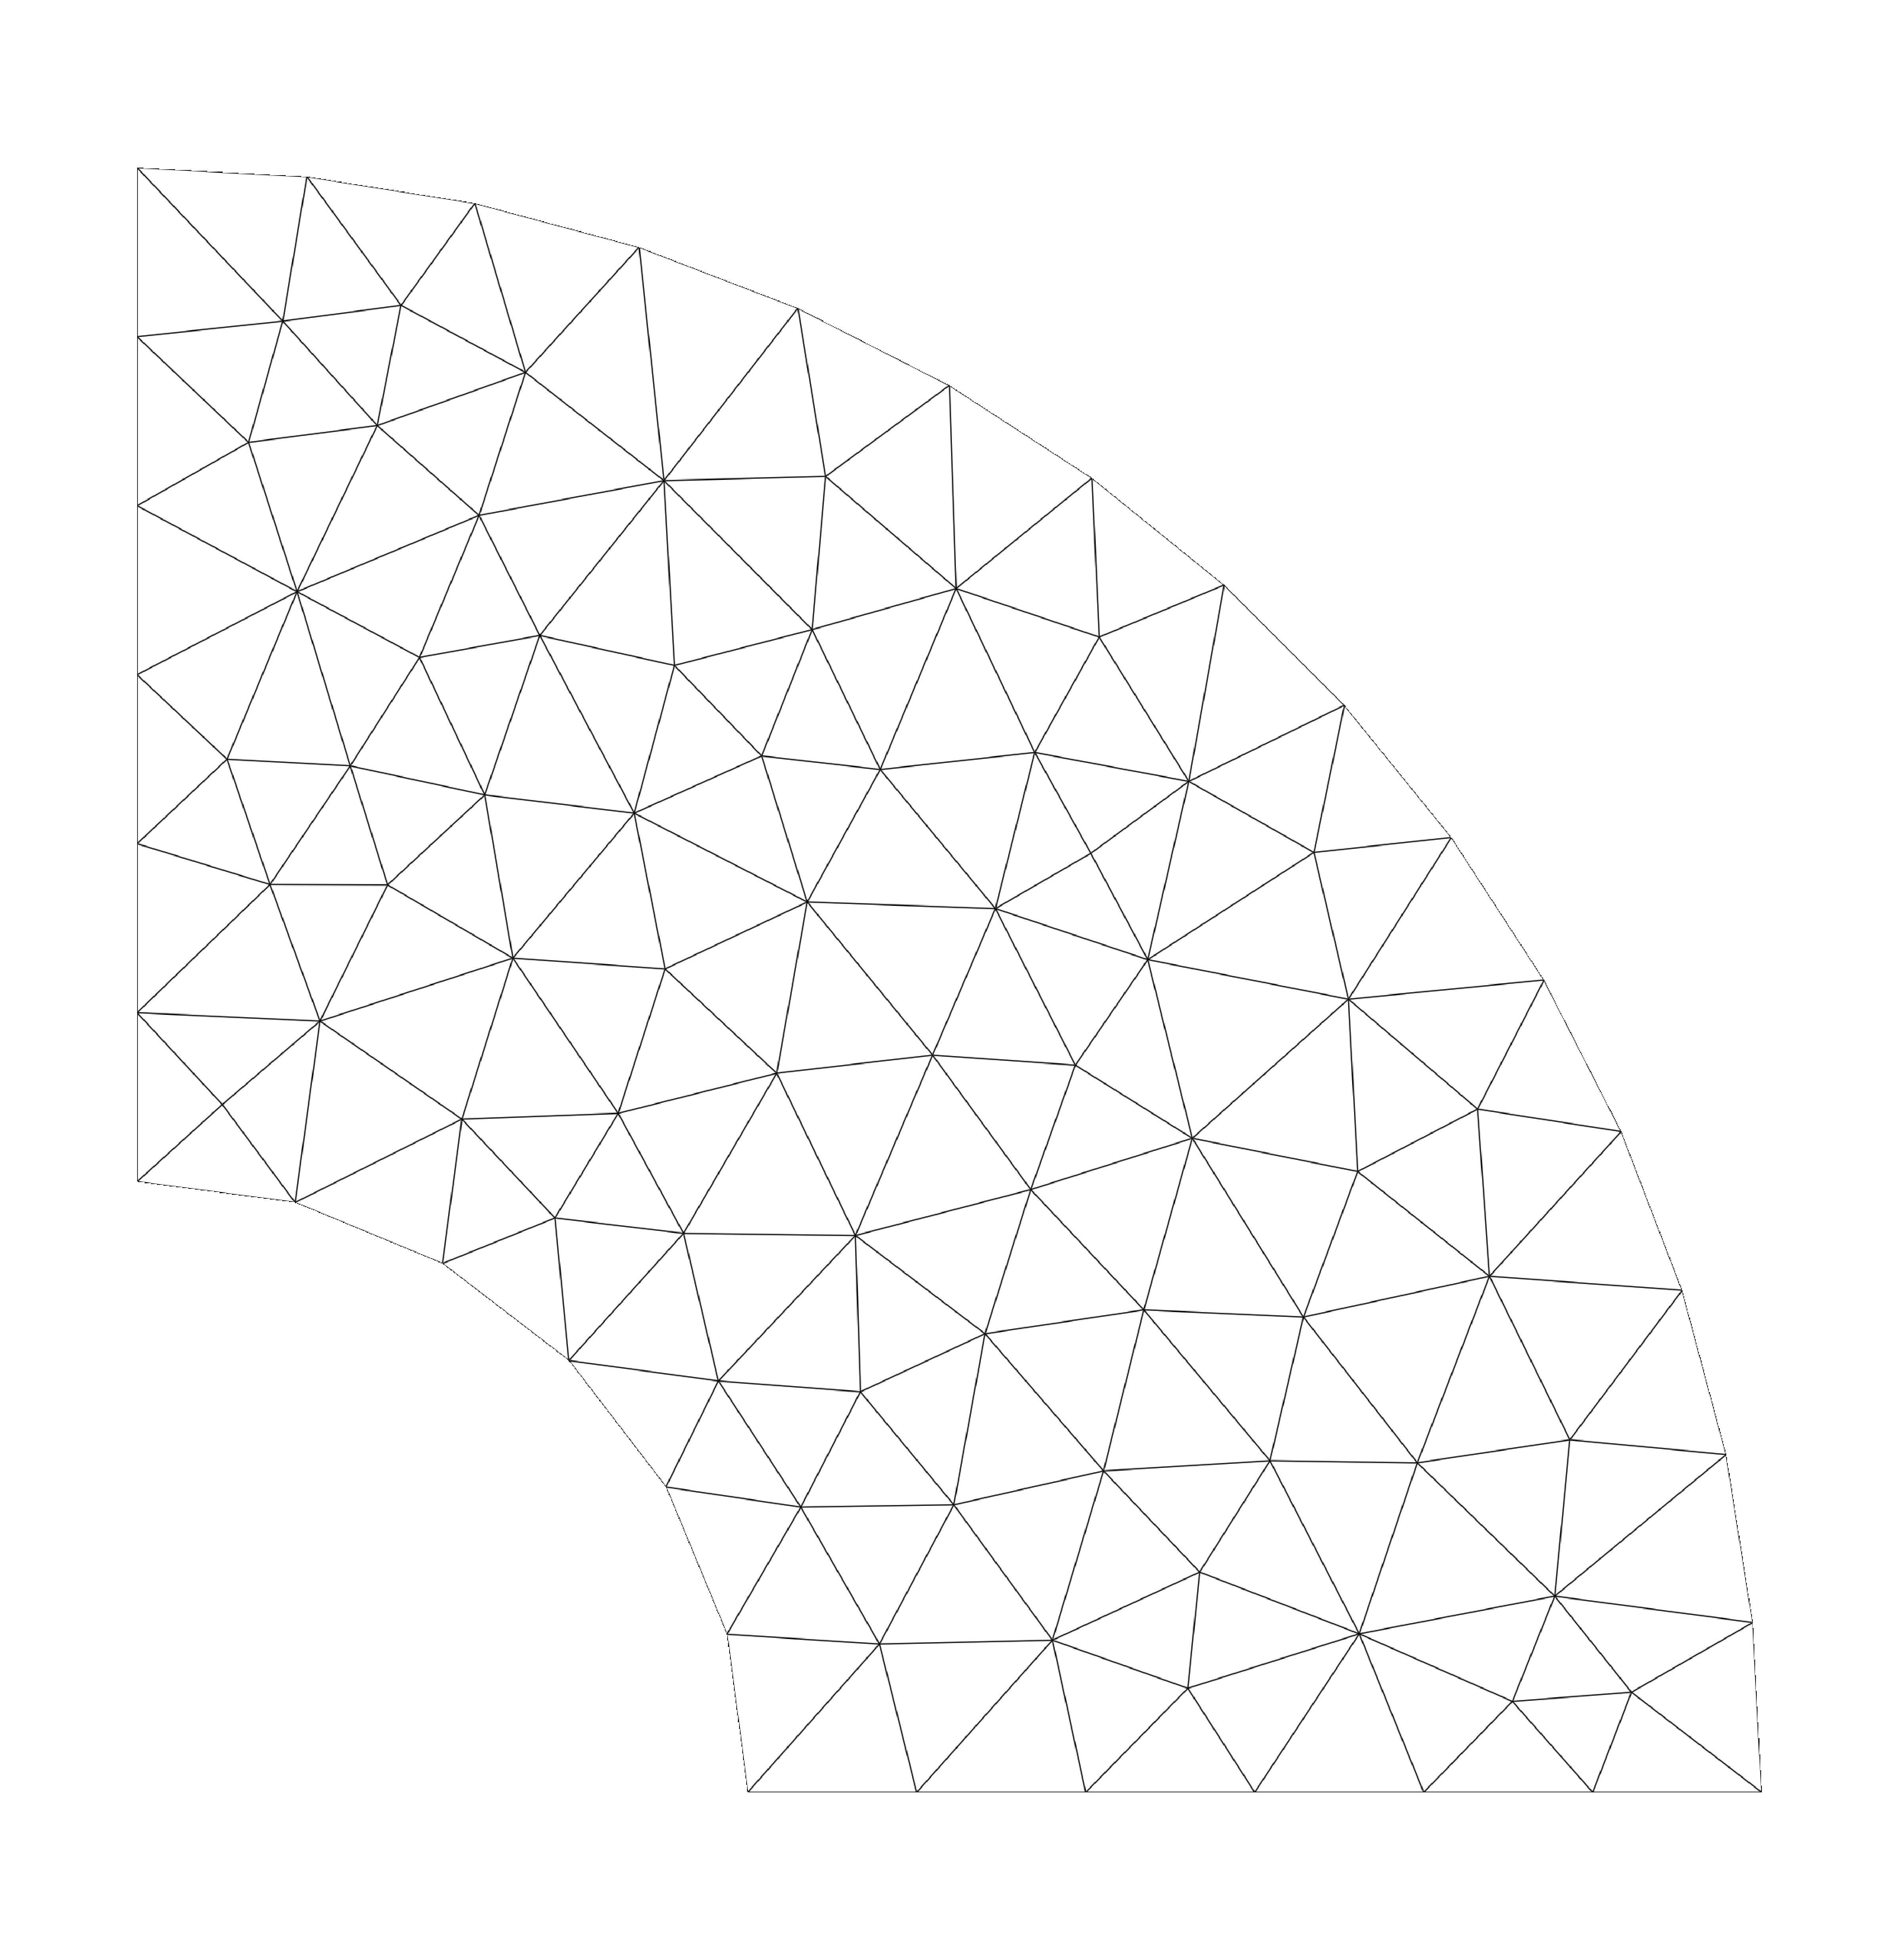
\includegraphics[scale=0.053]{figures/pressurisedCylinder-mesh} 
    }
 	\caption{Plate hole case geometry and mesh}
 	\label{fig:plateHole}
\end{figure}


\begin{figure}[H]
 	\centering
	\subfigure[Displacement convergence]
 	{
 		\label{fig:plateHole-disp:a}
    	\includegraphics[scale=0.8]{figures/pressurisedCylinder-dispErrors_tet} 
    }
 	\subfigure[Stress convergence]
 	{
 		\label{fig:plateHole-disp:b}
    	\includegraphics[scale=0.8]{figures/pressurisedCylinder-stressErrors_tet}  
    }
 	\caption{Pressurised cylinder case: displacement and stress magnitude discretisation errors for linear elastic material}
 	\label{fig:plateHole-disp}
 \end{figure}

%
%------------------------------------------------------------------------------
\subsubsection{Case 4: Cooks membrane}
%------------------------------------------------------------------------------
%


%
%------------------------------------------------------------------------------
\subsubsection{Case 4: Plate hole}
%------------------------------------------------------------------------------
%
% Case can be also found in:
% Finite volume method for stress analysis in complex domain
% Application of the nite volume method and unstructured meshes to linear elasticity
%
This benchmark problem consists of a thin, infinitely large plate with a circular hole, subjected to uniaxial tension. Owing to the symmetry of the geometry and loading, only one quarter of the plate is modeled as a finite domain. To minimize the influence of the finite computational boundaries, the exact tractions obtained from the analytical solution \cite{Demirdzic1997} are prescribed on the outer edges BC and CD. Symmetry boundary conditions are applied on boundaries AB and DE, while zero traction is specified on the hole boundary. The material properties are defined by a Young’s modulus of $E = 200 \,\text{GPa}$ and a Poisson’s ratio of $\nu = 0.3$.
%
\begin{figure}[H]
 	\centering
 	\subfigure[Case geometry]
 	{
 		\label{fig:plateHole:a}
    		\includegraphics[scale=1]{figures/plateHole-geometry} 
    }
	\subfigure[Hexahedral mesh]
 	{
 		\label{fig:plateHole:b}
    		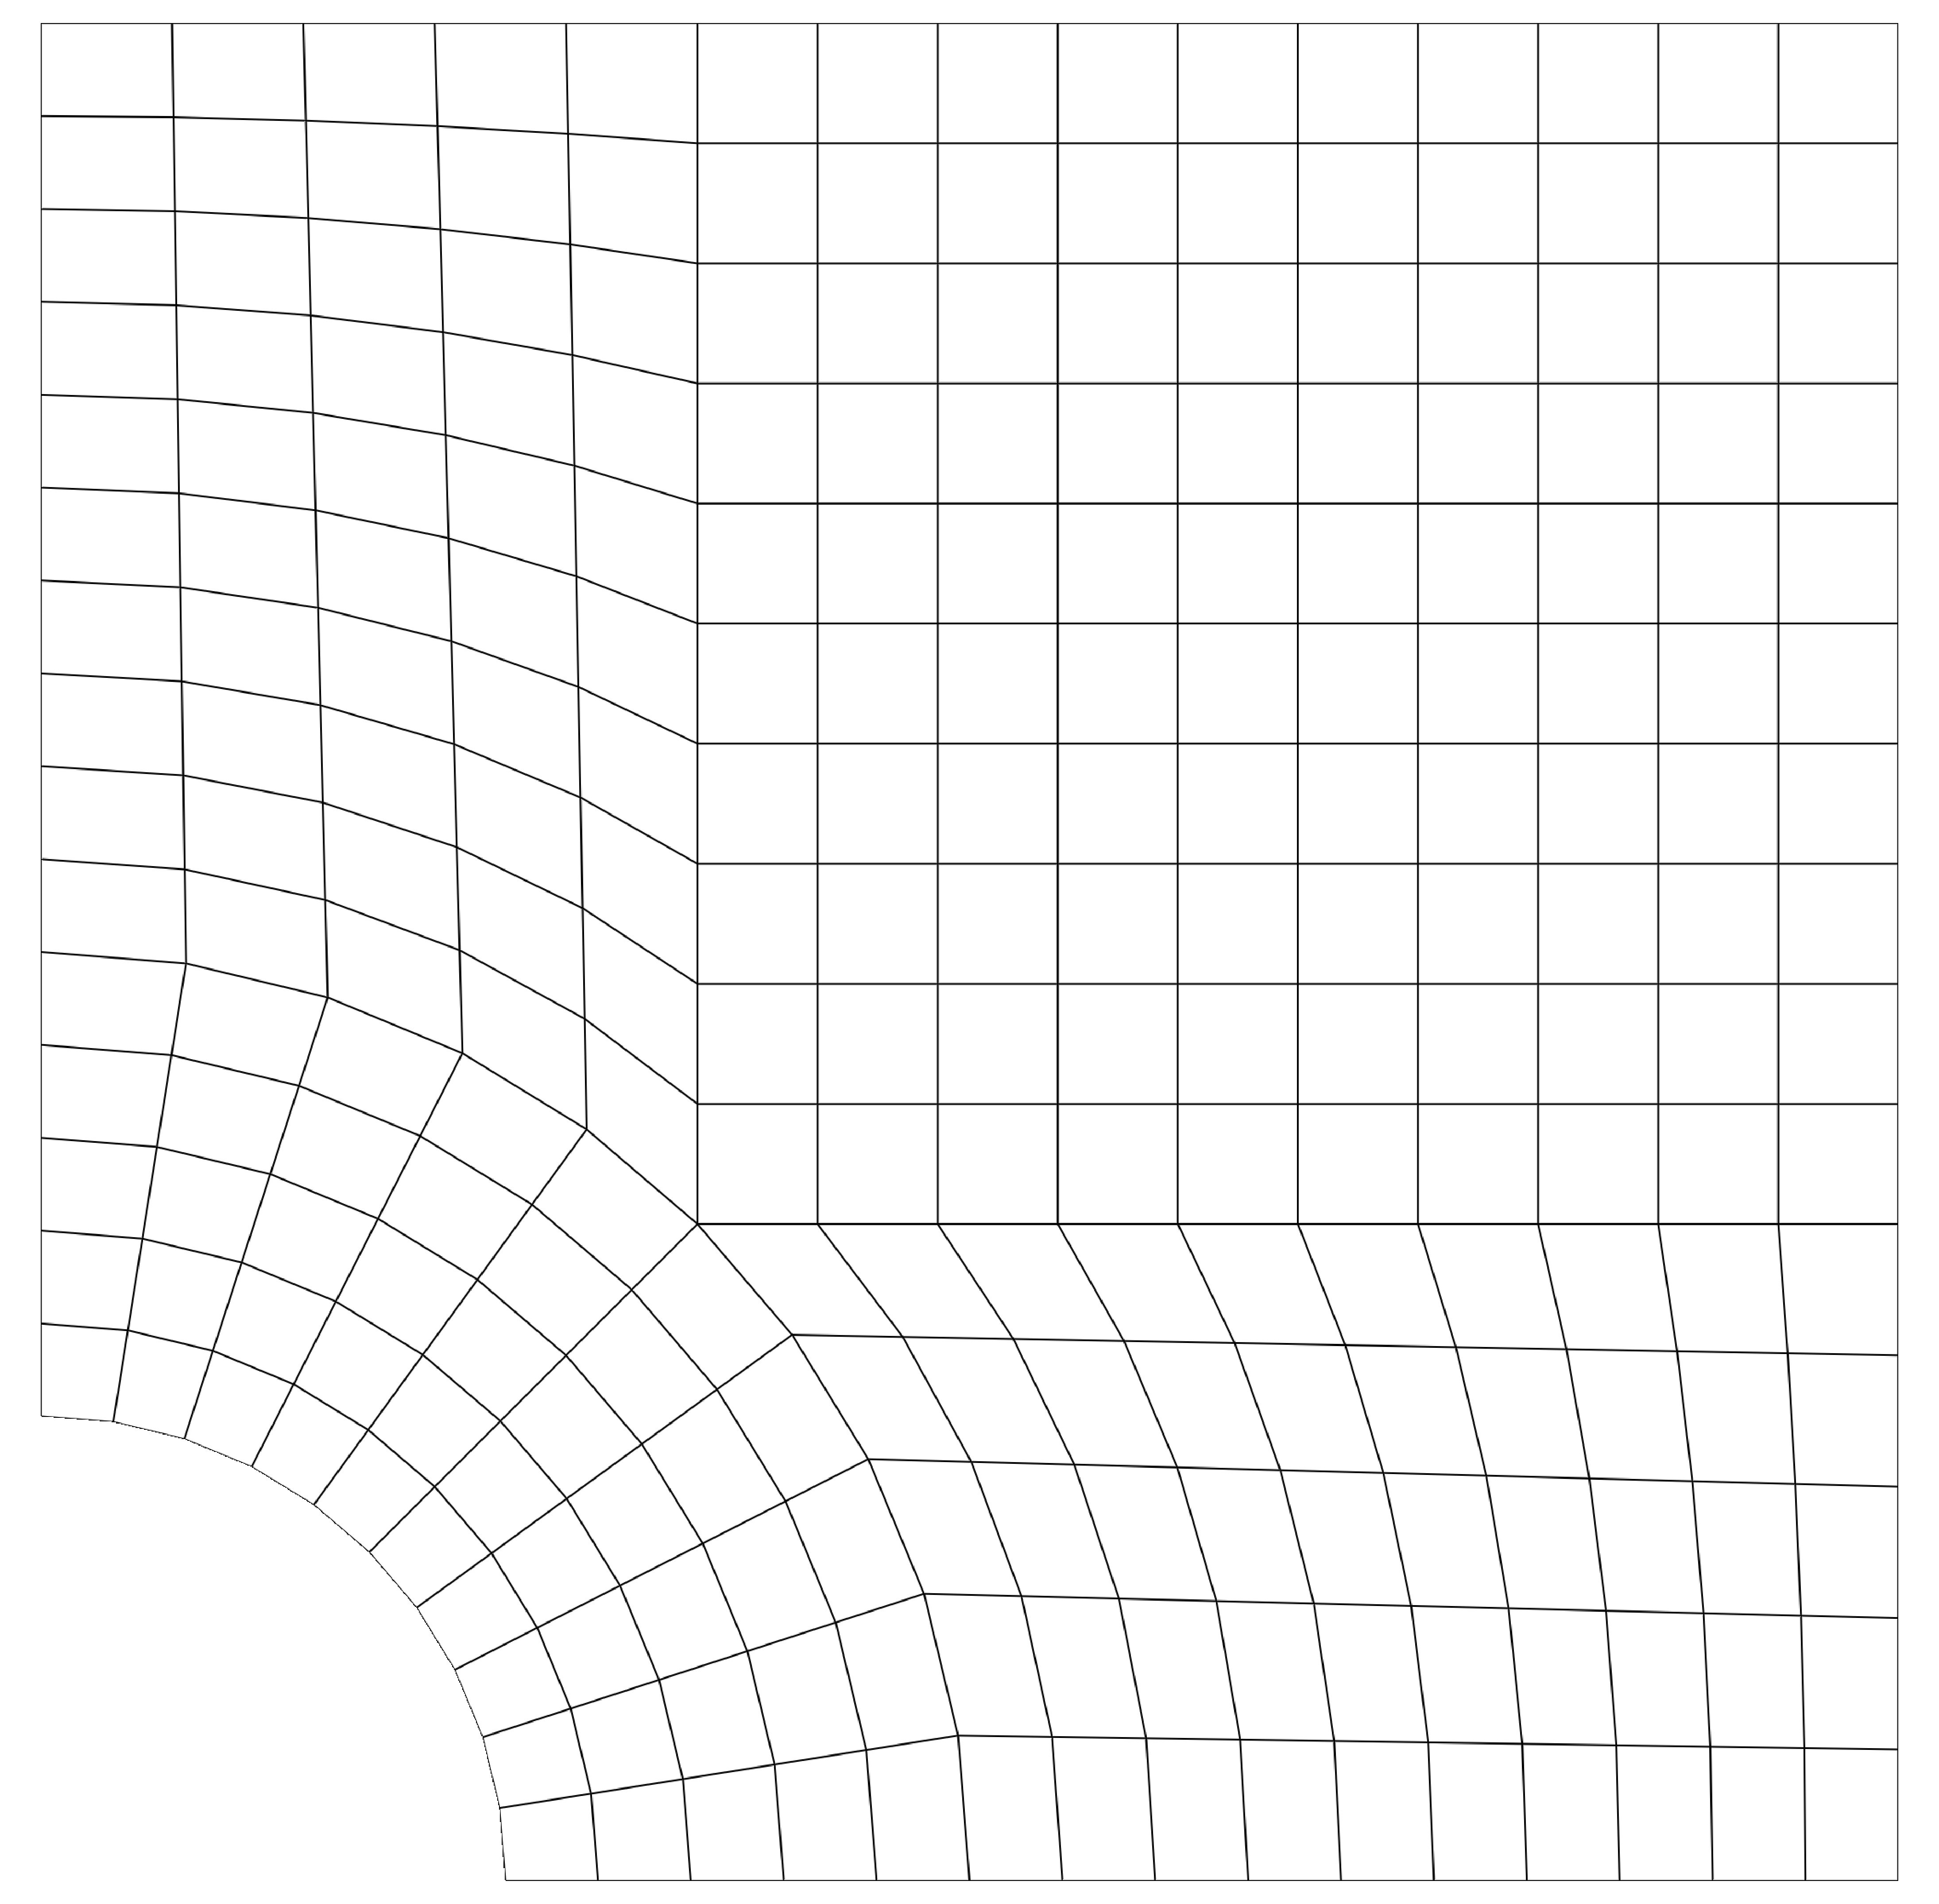
\includegraphics[scale=0.06]{figures/plateHole-hexmesh} 
    }
 	\subfigure[Tetrahedral mesh]
 	{
 		\label{fig:plateHole:a}
    	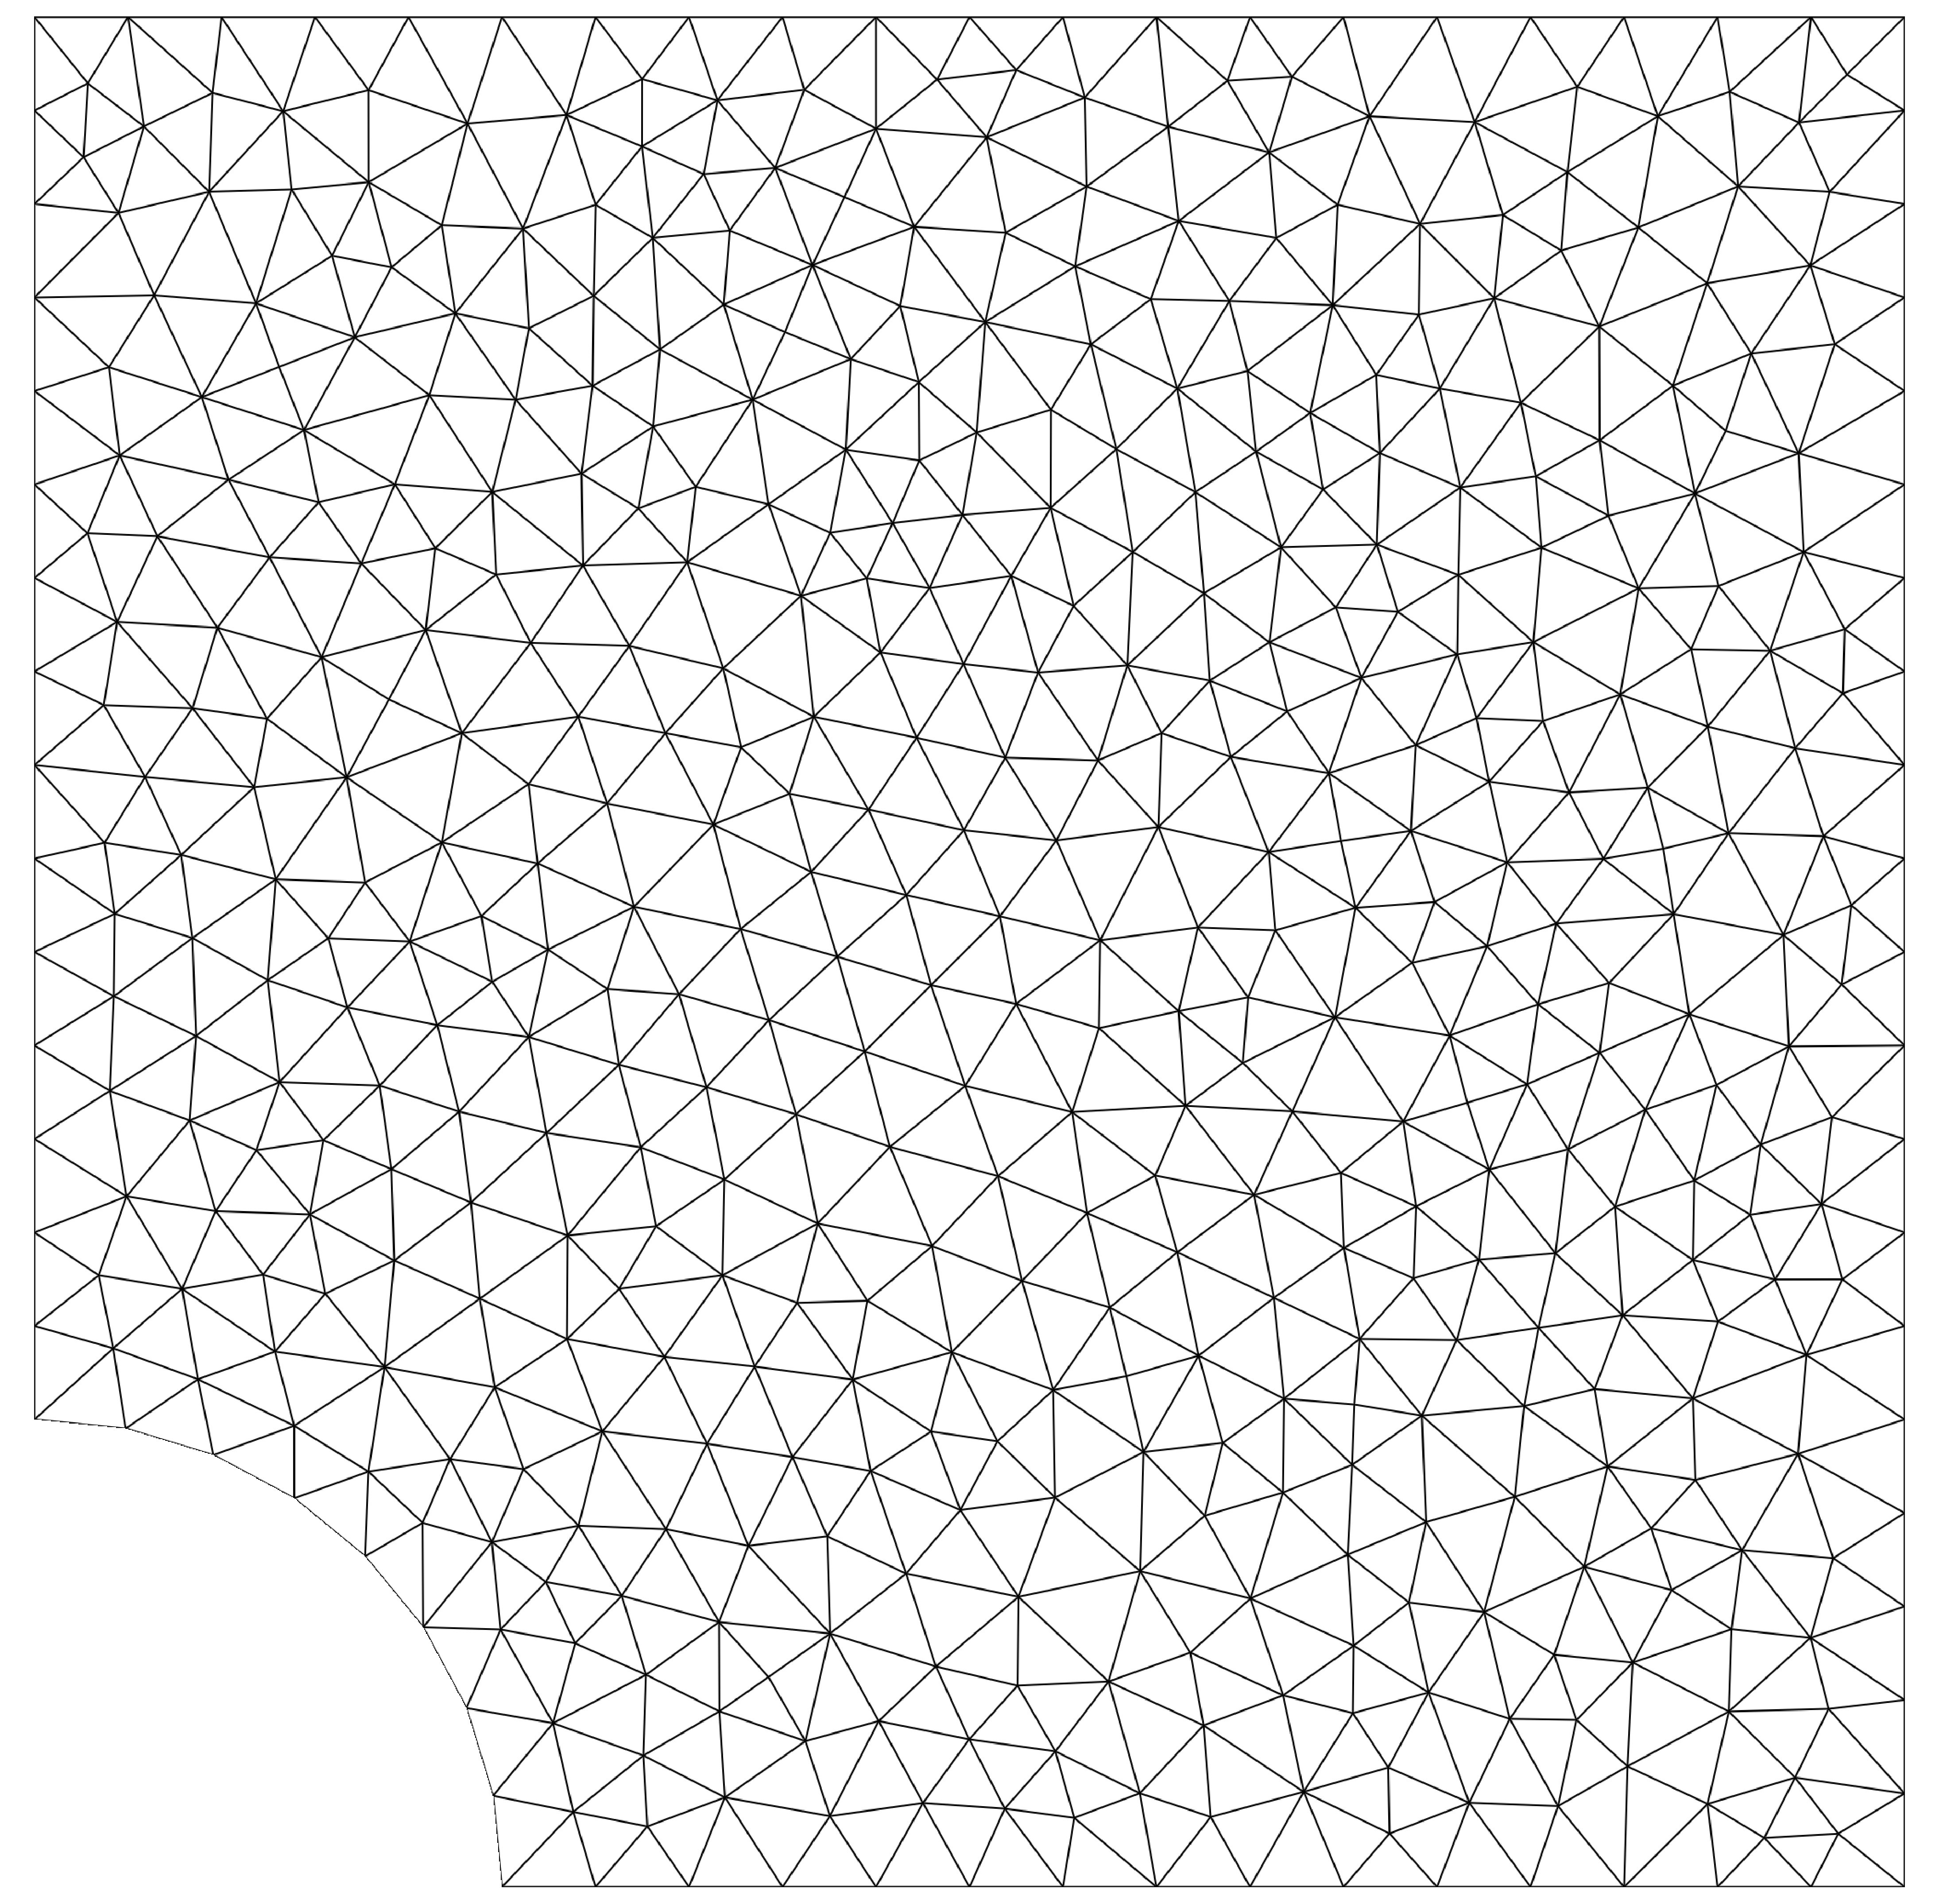
\includegraphics[scale=0.06]{figures/plateHole-tetmesh}  
    }
 	\caption{Plate hole case geometry and mesh}
 	\label{fig:plateHole}
\end{figure}
%
Hexahedral mesh with N3 needs 20 neighbours to avoid ill conditioning. This results in lower slope for displacement but not affecting the stresses. I'm not sure why S4F results flatten on finer meshes.
%
\begin{figure}[H]
 	\centering
	\subfigure[Hexahedral mesh]
 	{
 		\label{fig:plateHole-disp:a}
    	\includegraphics[scale=0.8]{figures/plateHole-dispErrors_hex} 
    }
 	\subfigure[Tetrahedral mesh]
 	{
 		\label{fig:plateHole-disp:b}
    	\includegraphics[scale=0.8]{figures/plateHole-dispErrors_tet-unstruct}  
    }
 	\caption{Plate hole case: displacement magnitude discretisation errors}
 	\label{fig:plateHole-disp}
 \end{figure}
 
\begin{figure}[H]
 	\centering
	\subfigure[Hexahedral mesh]
 	{
 		\label{fig:plateHole-stress:a}
    	\includegraphics[scale=0.8]{figures/plateHole-stressErrors_hex} 
    }
 	\subfigure[Tetrahedral mesh]
 	{
 		\label{fig:plateHole-stress:a}
    	\includegraphics[scale=0.8]{figures/plateHole-stressErrors_tet-unstruct}  
   	}
 	\caption{Plate hole case: $\sigma_{xx}$, $\sigma_{yy}$, $\sigma_{xy}$ stress discretisation errors.}
 	\label{fig:plateHole-stress}
 \end{figure}
 
 
%
%------------------------------------------------------------------------------
\subsubsection{Case 5: Elliptic plate}
%------------------------------------------------------------------------------
%

%
%------------------------------------------------------------------------------
\subsubsection{Case 6: Spherical cavity}
%------------------------------------------------------------------------------
%

%
%------------------------------------------------------------------------------
\subsubsection{Case 7: Idealised ventricle}
%------------------------------------------------------------------------------
%

%
%------------------------------------------------------------------------------
\subsection{Error-cost relationship}
%------------------------------------------------------------------------------
%
An additional clarification regarding the notation used in the next sections is needed. The abbreviations are as follows: “$S4F^{seg}$” stands for solids4foam segregated solver whereas “$S4F^{snes}$” is the same solver with JFNK algorithm. Both solvers are second-order accurate, meaning that their accuracy is comparable with high-order discretisation with p=1.
%
%------------------------------------------------------------------------------
\subsection{Stabilisation scheme effects}
%------------------------------------------------------------------------------
%

%
%------------------------------------------------------------------------------
\subsection{Effects of poor interpolation conditioning}
%------------------------------------------------------------------------------
%


%
%------------------------------------------------------------------------------
\subsection{Different choice for approximate Jacobian}
%------------------------------------------------------------------------------
%

Plate hole sa hex mrezom tu staviti i objasniti sto se desava u 2D-u sa kondicijskim brojem interpolacije

\subsection{Code parallelisation}

%%%%%%%%%%%%%%%%%%%%%%%%%%%%%%%%%%%%%%%%%%%%%%%%%%%%%%%%%%%%%%%%%%
\section{Conclusions} \label{sec:conclusion}
%%%%%%%%%%%%%%%%%%%%%%%%%%%%%%%%%%%%%%%%%%%%%%%%%%%%%%%%%%%%%%%%%%
%% A Jacobian-free Newton-Krylov solution algorithm has been proposed for solid mechanics problems discretised using the cell-centred finite volume method.
%% A compact-stencil discretisation of the diffusion term is proposed as the preconditioner matrix, allowing a straightforward extension of existing segregated solution frameworks.
%% The key conclusions of the work are:
%% \begin{itemize}
%% 	\item \textbf{Efficiency of Jacobian-free Newton-Krylov approach}: The proposed Jacobian-free Newton-Krylov solution algorithm has been shown to be faster than a conventional segregated solution algorithm for all linear and nonlinear elastic test cases examined. In particular, speedups of one order of magnitude were seen in many cases, with a maximum speedup of 341 in the 2-D linear elastic Cook's membrane case.

%% 	\item \textbf{Additional memory overhead}: The Jacobian-free Newton-Krylov approach has been shown to have approximately the same memory requirements as a segregated solution algorithm for less than $10^4$ degrees of freedom, but generally increases beyond this.
%% 	The greatest memory increase was found to be 3.6 and occured in the spherical cavity case. Nonetheless, these differences are likely attributed to the different linear solver and preconditioner used in the Jacobian-free Newton-Krylov approach (GMRESS with multigrid or LU decomposition) compared to the segregated approach (conjugate gradient with zero in-fill Cholesky decomposition).
	
%% 	\item \textbf{Applicability to existing segregated frameworks}: By employing a compact-stencil diffusion approximation of the Jacobian as the preconditioner, the proposed Jacobian-free Newton-Krylov approach can be integrated into existing segregated finite volume frameworks with minimal modifications to the existing code base, in particular if existing publicly available Jacobian-free Newton-Krylov solvers (e.g., PETSc) are used.

%% %	\item \textbf{Benchmark performance}: On a range of benchmark cases, the method maintained accuracy and robustness across different dimensions, geometries, and material behaviours, proving its versatility.

%% 	\item \textbf{Choice of preconditioning approach}: It has been shown that the LU direct solver preconditioning approach is faster than multigrid and ILU($k$) approaches for 2-D cases and moderately-sized 3-D problems; however, for larger 3-D problems the multigrid approach is the fastest while also requiring less memory than the direct LU approach. In addition, the multigrid approach is seen to show approximate ideal scaling in a parallel strong scaling study.
	
%% 	\item \textbf{Rhie-Chow stabilisation}: The magnitude of the Rhie-Chow stabilisation term is shown to affect the speed and robustness of the Jacobian-free Newton-Krylov approach, where $\alpha = 0.1$ and $1$ are seen to outperform $\alpha = 0.01$.

%% 	\item \textbf{Open access and extensibility}: The implementation is made publicly available within the solids4foam toolbox for OpenFOAM to encourage implementation critique, community adoption, and comparative studies, contributing to advancing finite volume solid mechanics simulations.
%% \end{itemize}

%% %Future work:
%% %- Modifying the compact preconditioner matrix to account for plasticity would allow the method to work in the failed cases, but this will be left for future studies.
%% %- Including non-orthogonality in the preconditioner.
%% %- Compare with a full Jacobian approach:  avoids the storage and computational costs associated with forming the full Jacobian matrix, offering significant advantages for large-scale and complex problems.
%% %- Use Picard as initial step for JFNK: It is not sufficiently robust: this can be seen in some of the test cases where it diverges, e.g hyperelastic cases. In other cases, convergence is quick so initialisation is not needed. So Picard could work if made more robust (maybe add pseudo time). Add this comment to the conclusions.
%% %- Higher-order discretisations, where the same compact preconditioning matrix is used
%% %- Monolithic FSI framework, where both fluid and solid are solved in a monolithic JFNK manner

%% The presented study highlights the potential of the Jacobian-free Newton-Krylov method in finite-volume solid mechanics simulations, yet several areas for future exploration remain:
%% \begin{enumerate}
%% 	\item{Enhanced preconditioning for plasticity}: While the proposed \emph{elastic} compact-stencil preconditioning matrix has been shown to perform well in linear and nonlinear elastic scenarios, it fails in cases exhibiting plasticity, where a segregated approach succeeds. Future studies will explore modifications to the compact preconditioning matrix to extend the applicability of the proposed approach to small and large strain elastoplasticity.

%% 	\item{Incorporation of non-orthogonality in the preconditioner}: The current preconditioning matrix does not account for non-orthogonal contributions in distorted meshes. Including these effects in future work could further enhance robustness, particularly for complex geometries.

%% 	\item{Comparison with full Jacobian approaches}: A comparison with a fully coupled Jacobian-based method would provide greater insights into the trade-offs between computational cost, memory usage, and convergence performance. Such a study could highlight the specific advantages of the Jacobian-free Newton-Krylov approach for large-scale, nonlinear problems.

%% 	\item{Globalisation strategies}: The robustness and efficiency of the proposed Jacobian-free Newton-Krylov approach could be improved for nonlinear problems by using a segregated approach as an initialisation phase for each loading step. In its current form, the segregated approach would not be generally suitable as it is less robust on several nonlinear hyperelastic problems; however, modifications such as introducing pseudo-time-stepping (introducing a pseudo-time damping term), may enhance its robustness and suitability for these scenarios.

%% 	\item{Higher-order discretisations}: Future work will explore the application of the proposed linear elastic compact-stencil Jacobian-free Newton-Krylov approach to higher-order finite volume discretisations. Using the same compact-stencil preconditioning matrix for these discretisations could yield efficient and accurate solutions for problems requiring increased fidelity.

%% 	\item{Development of a monolithic fluid-solid interaction framework}: Extending the Jacobian-free Newton-Krylov method to a fully monolithic fluid-solid interaction framework presents a promising avenue. In this approach, both fluid and solid domains would be solved simultaneously using a unified Jacobian-free Newton-Krylov method, potentially improving stability and performance in highly nonlinear coupled problems.
%% \end{enumerate}



%%%%%%%%%%%%%%%%%%%%%%%%%%%%%%%%%%%%%%%%%%%%%%%%%%%%%%%%%%%%%%%%%%%%%%%%%%%%%%%
\backmatter
%
%%%%%%%%%%%%%%%%%%%%%%%%%%%%%%%%%%%%%%%%%%%%%%%%%%%%%%%%%%%%%%%%%%%%%%%%%%%%%%%
\bmhead{Data Availability}
%%%%%%%%%%%%%%%%%%%%%%%%%%%%%%%%%%%%%%%%%%%%%%%%%%%%%%%%%%%%%%%%%%%%%%%%%%%%%%%
%
The codes presented are publicly available at \url{https://github.com/solids4foam/solids4foam}, and the cases and plotting scripts are available at \url{https://github.com/solids4foam/solid-benchmarks}.
%
%%%%%%%%%%%%%%%%%%%%%%%%%%%%%%%%%%%%%%%%%%%%%%%%%%%%%%%%%%%%%%%%%%%%%%%%%%%%%%%
\bmhead{Declaration of generative AI and AI-assisted technologies in the writing process}
%%%%%%%%%%%%%%%%%%%%%%%%%%%%%%%%%%%%%%%%%%%%%%%%%%%%%%%%%%%%%%%%%%%%%%%%%%%%%%%
%
During the preparation of this work, the authors used ChatGPT and Grammarly as writing assistants.
After using these tools, the authors reviewed and edited the content as needed and take full responsibility for the content of the publication.
%
%%%%%%%%%%%%%%%%%%%%%%%%%%%%%%%%%%%%%%%%%%%%%%%%%%%%%%%%%%%%%%%%%%%%%%%%%%%%%%%
\bmhead{Acknowledgments}
%%%%%%%%%%%%%%%%%%%%%%%%%%%%%%%%%%%%%%%%%%%%%%%%%%%%%%%%%%%%%%%%%%%%%%%%%%%%%%%
%
This project has received funding from the European Research Council (ERC) under the European Union’s Horizon 2020 research and innovation programme (Grant Agreement No. 101088740).
Financial support is gratefully acknowledged from the Irish Research Council
through the Laureate programme, grant number IRCLA/2017/45, from Bekaert through
the University Technology Centre (UTC phases I and II) at UCD
(www.ucd.ie/bekaert), from I-Form, funded by Science Foundation Ireland (SFI)
Grant Numbers {16/RC/3872} and {21/RC/10295\_P2}, co-funded under European Regional Development Fund and by I-Form industry partners, and from NexSys, funded by SFI Grant Number 21/SPP/3756.
Additionally, the authors wish to acknowledge the DJEI/DES/SFI/HEA Irish Centre for High-End Computing (ICHEC) for the provision of computational facilities and support (www.ichec.ie), and part of this work has been carried out using the UCD ResearchIT Sonic cluster which was funded by UCD IT Services and the UCD Research Office.
%
\newpage
%
\begin{appendices}
%
%%%%%%%%%%%%%%%%%%%%%%%%%%%%%%%%%%%%%%%%%%%%%%%%%%%%%%%%%%%%%%%%%%%%%%%%%%%%%%%
%
\section{Mechanical Laws}
\label{app:mechLaws}
%
%%%%%%%%%%%%%%%%%%%%%%%%%%%%%%%%%%%%%%%%%%%%%%%%%%%%%%%%%%%%%%%%%%%%%%%%%%%%%%%
%
\subsection{Linear Elasticity}
The definition of engineering stress $\bb{\sigma}_s$ for linear elasticity can be given as
\begin{eqnarray}  \label{eq:linearElastic}
	\bb{\sigma}_s
	&=& 2 \mu \bb{\varepsilon} + \lambda \, \text{tr} \left( \bb{\varepsilon} \right) \textbf{I} \notag \\
	&=& \mu \bb{\nabla} \bb{u} + \mu \left( \bb{\nabla} \bb{u}\right)^{\text{T}} + \lambda \left(\bb{\nabla} \cdot \bb{u} \right) \textbf{I}
\end{eqnarray}
where $\lambda$ is the first Lam\'{e} parameter, and $\mu$ is the second Lam\'{e} parameter, synonymous with the shear modulus.
The Lam\'{e} parameters can be expressed in term of the Young's modulus ($E$) and Poisson's ratio $\nu$ as
\begin{eqnarray}
	\mu = \frac{E}{2(1 + \nu)}, \quad \lambda = \frac{E \nu}{(1+\nu)(1 - 2\nu)}
\end{eqnarray}
%
%------------------------------------------------------------------------------
\subsection{St.\,Venant-Kirchoff Hyperelasticity}
%------------------------------------------------------------------------------
%
The St.\,Venant-Kirchoff model defines the second Piola–Kirchhoff stress $\textbf{S}$ as
\begin{eqnarray}
	\bb{S} &=& 2 \mu \bb{E} + \lambda \, \text{tr} \left( \bb{E} \right) \textbf{I}
\end{eqnarray}
where, as before, $\lambda$ is the first Lam\'{e} parameter, and $\mu$ is the second Lam\'{e} parameter.
The Lagrangian Green strain $\textbf{E}$ is defined as
\begin{eqnarray}
	\bb{E} &=& \frac{1}{2} \left( \bb{\nabla} \bb{u} + \bb{\nabla} \bb{u}^{\text{T}} + \bb{\nabla} \bb{u} \cdot \bb{\nabla} \bb{u}^{\text{T}}  \right)
\end{eqnarray}

The true stress can be calculated from the second Piola–Kirchhoff stress as
\begin{eqnarray} \label{eq:S2sigma}
	\bb{\sigma} &=& \frac{1}{J} \bb{F} \cdot \bb{S} \cdot \bb{F}^{\text{T}}
\end{eqnarray}
%
%------------------------------------------------------------------------------
\subsection{Neo-Hookean Hyperelasticity}
%------------------------------------------------------------------------------
%
The definition of true (Cauchy) stress $\bb{\sigma}$ for neo-Hookean hyperelasticity can be given as
\begin{eqnarray} \label{eq:neoHook}
	\bb{\sigma}
	&=& \frac{\mu}{J} \, \text{dev} \left( \bar{\bb{b}} \right) + \frac{\kappa}{2} \frac{J^2 - 1}{J} \textbf{I}
\end{eqnarray}
where, once again, $\mu$ is the shear modulus, and $\kappa$ is the bulk modulus.
The bulk modulus can be expressed in terms of the Young's modulus ($E$) and Poisson's ratio $\nu$ as
\begin{eqnarray}
	\kappa = \frac{E}{3(1 - 2\nu)}
\end{eqnarray}
The volume-preserving component of the elastic left Cauchy--Green deformation tensor is $\boldsymbol{b}$ is given as
\begin{eqnarray}
	\bar{\bb{b}} = J^{-2/3} \bb{b} = J^{-2/3} \bb{F} \cdot \bb{F}^{\text{T}}
\end{eqnarray}
In the limit of small deformations $\lVert \nabla \mathbf{u} \rVert  \ll 1$, neo-Hookean hyperelasticity (Equation \ref{eq:neoHook}) reduces to linear elasticity (Equation \ref{eq:linearElastic}).
%
%------------------------------------------------------------------------------
\subsection{Guccione Hyperelasticity}
%------------------------------------------------------------------------------
%
The \citet{Guccione1995} hyperelastic law defines the second Piola-Kirchhoff stress as
\begin{eqnarray}
	\boldsymbol{S}
		%&=&  \frac{\partial \Psi}{\partial \boldsymbol{E} } \notag \\
		&=& \frac{\partial Q}{\partial \boldsymbol{E} } \left( \frac{C}{2} \right) e^Q + \frac{\kappa}{2} \frac{J^2 - 1}{J} \textbf{I} 
\end{eqnarray}
where
\begin{eqnarray}
%	\Psi(I_1, I_2, I_4, I_5) &=& \frac{C}{2} \left( e^{Q(I_1, I_2, I_4, I_5)} - 1 \right) \\
	Q(I_1, I_2, I_4, I_5) &=& c_t I_1^2 - 2 c_t I_2 + (c_f - 2c_{fs} + c_t) I_4^2   + 2(c_{fs} - c_t) I_5 \\
	\frac{\partial Q}{\partial \boldsymbol{E} }
%		&=& \frac{\partial Q}{\partial I_1} \frac{\partial I_1}{\partial \boldsymbol{E} } + \frac{\partial Q}{\partial I_2} \frac{\partial I_2}{\partial \boldsymbol{E} }
%		+ \frac{\partial Q}{\partial I_4} \frac{\partial I_4}{\partial \boldsymbol{E} } + \frac{\partial Q}{\partial I_5} \frac{\partial I_5}{\partial \boldsymbol{E} } \notag \\
		&=&  2 c_t \boldsymbol{E} + 2(c_f - 2 c_{fs} + c_t)I_4 ( \boldsymbol{f_0} \otimes \boldsymbol{f_0} ) \notag \\
		&&+ 2(c_{fs} - c_t)\left[\boldsymbol{E} \cdot  (\boldsymbol{f_0} \otimes \boldsymbol{f_0}) + ( \boldsymbol{f_0} \otimes \boldsymbol{f_0} ) \cdot \boldsymbol{E} \right]
\end{eqnarray}
The scalars $C$, $c_f$, $c_{fs}$, and $c_t$ are material parameters and invariants of the Green strain, $\boldsymbol{E} = \boldsymbol{F}^{\text{T}} \cdot \boldsymbol{F}$, are defined as
\begin{eqnarray}
	I_1 = \text{tr}(\boldsymbol{E}), \quad
	I_2 =  \frac{1}{2} \left[ \text{tr}^2(\boldsymbol{E}) - \text{tr}(\boldsymbol{E} \cdot \boldsymbol{E}) \right], \notag \\
	I_4 = \boldsymbol{E}  : \left( \boldsymbol{f_0} \otimes \boldsymbol{f_0} \right), \quad 
	I_5 = \left( \boldsymbol{E} \cdot \boldsymbol{E} \right): \left( \boldsymbol{f_0} \otimes \boldsymbol{f_0} \right)
\end{eqnarray}
with $\boldsymbol{f_0}$ representing the unit fibre directions in the initial configuration.

Equation \ref{eq:S2sigma} is used to convert the second Piola-Kirchhoff stress to the true stress.
%
%------------------------------------------------------------------------------
\subsection{Mon-Rivlin - add here if used}
%------------------------------------------------------------------------------
%

%
%%%%%%%%%%%%%%%%%%%%%%%%%%%%%%%%%%%%%%%%%%%%%%%%%%%%%%%%%%%%%%%%%%%%%%%%%%%%%%%
%
\section{Preconditioner Based on True Jacobian} 
\label{app:P}
%
%%%%%%%%%%%%%%%%%%%%%%%%%%%%%%%%%%%%%%%%%%%%%%%%%%%%%%%%%%%%%%%%%%%%%%%%%%%%%%%
%

\begin{equation}
\begin{split} 
& \sum_{f \,\in\, \mathcal{F}_P^{\text{int}}} \bb{n}_{f} \cdot \left[  \sum_{q=1}^{q=N_{f,q}}\alpha_q \; (\bb{\sigma}_s)_{f,q} \right] \Gamma_f 
= \\
=&
\sum_{f \,\in\, \mathcal{F}_P^{\text{int}}} \bb{n}_{f} \cdot \left [ \sum_{q=1}^{q=N_{f,q}}\alpha_q \; \left(\mu (\nabla \bb{u})_{f,q} + \mu (\nabla \bb{u})^T_{f,q} +\lambda \text{tr}((\nabla \bb{u})_{f,q} )\mathbf{I}\right) \right]\Gamma_f \\
=& 
\sum_{f \,\in\, \mathcal{F}_P^{\text{int}}} \left [ \sum_{q=1}^{q=N_{f,q}}\alpha_q \; \left(\mu \sum_{N\,\in\,\mathcal{S}_f}(\bb{c}_{x_N}\cdot \bb{n}_f)\mathbf{I} \bb{u}_N  + \mu \sum_{N\,\in\,\mathcal{S}_f}(\bb{c}_{x_N}\bb{n}_f^T) \bb{u}_N +\lambda  \sum_{N\,\in\,\mathcal{S}_f}(\bb{n}_f \bb{c}_{x_N}^T) \bb{u}_N\right) \right]\Gamma_f
\end{split}
\end{equation}


\textcolor{red}{Provjeri sto se desava sa simetrijom i displacement rubom pa nadopisi}

\begin{equation}
\begin{split}
&\oint_{\Gamma_P} \bb{n} \cdot \bb{\sigma}_s \; \text{d}\Gamma_P  
=
\sum_{f \, \in \,\mathcal{F}_P} \int_{\Gamma_f} \bb{n} \cdot \bb{\sigma}_s \; \text{d}\Gamma_f 
\approx 
\sum_{f \,\in\, \mathcal{F}_P^{\text{int}}} \bb{n}_{f} \cdot \left [ \sum_{q=1}^{q=N_{f,q}}\alpha_q \; (\bb{\sigma}_s)_{f,q} \right]\Gamma_f \\
& + \sum_{b\, \in \,\mathcal{F}_P^{\text{non-trac}}}  \bb{n}_{b} \cdot \left [ \sum_{q=1}^{q=N_{f,q}}\alpha_q \; (\bb{\sigma}_s)_{b,q} \right]\Gamma_b 
+ \sum_{b\, \in \, \mathcal{F}_P^{\text{trac}}}   \bb{n}_{b} \cdot  \sum_{q=1}^{q=N_{f,q}}\bb{T}_{b,q} \Gamma_b,
\end{split}
\end{equation}
%
%%%%%%%%%%%%%%%%%%%%%%%%%%%%%%%%%%%%%%%%%%%%%%%%%%%%%%%%%%%%%%%%%%%%%%%%%%%%%%%
%
\section{High-order Derivatives} 
\label{app:derivatives}
%
%%%%%%%%%%%%%%%%%%%%%%%%%%%%%%%%%%%%%%%%%%%%%%%%%%%%%%%%%%%%%%%%%%%%%%%%%%%%%%%
%
The reconstruction of higher-order derivatives is performed for each component of the displacement vector field $\bb{u} = [u_x,\,u_y,\,u_z]^{\mathrm{T}}$.
Specifically, the Hessian $(\nabla \nabla \bb{u})$ and the third-order derivative tensor $(\nabla \nabla \nabla \bb{u})$ appearing in Equation \eqref{eq:alphaJump} are obtained by independently reconstructing the corresponding scalar derivatives of $u_x$, $u_y$, and $u_z$.

For a scalar field $u$ representing one displacement component, the Hessian at the cell centre $P$ is reconstructed as a weighted sum of the neighbouring cell values contained in the stencil $\mathcal{S}_P$:
\begin{equation}
(\nabla \nabla \bb{u})_P^{u}
= \sum_{N \in \mathcal{S}_P} \bb{c}_{{\bb{x}\bb{x}}_N} \phi_N,
\label{eq:hessianComponent}
\end{equation}
%
where $\bb{c}_{{\bb{x}\bb{x}}_N}$ is a symmetric second-order coefficient tensor:
%
\begin{equation}
\bb{c}_{{\bb{x}\bb{x}}_N} =
\begin{bmatrix}
c_{xx_N} & c_{xy_N} & c_{xz_N} \\
c_{xy_N} & c_{yy_N} & c_{yz_N} \\
c_{xz_N} & c_{yz_N} & c_{zz_N}
\end{bmatrix}.
\label{eq:thirdTensor}
\end{equation}
Coefficients in tensor $\bb{c}_{{\bb{x}\bb{x}}_N}$ are derived from the rows of the reconstruction matrix $\mathbf{\bar{A}}$ corresponding to the second-order monomials.
The complete displacement Hessian $(\nabla \nabla \bb{u})$ is assembled from the Hessians of its three scalar components.

For $p = 3$, the third-order derivative tensor $(\nabla \nabla \nabla u)_P$ for each displacement component is computed as:
%
\begin{equation}
(\nabla \nabla \nabla \bb{u})_P^u
= \sum_{N \in \mathcal{S}_P} \mathbf{c}_{\bb{x}\bb{x}\bb{x}_N} u_N,
\label{eq:thirdTensor}
\end{equation}
where $\mathbf{c}_{\bb{x}\bb{x}\bb{x}_N}$ is a symmetric third-order coefficient tensor $\mathbf{c}_{\bb{x}\bb{x}\bb{x}_N} =\big[c_{xxx_N},c_{xxy_N},c_{xxz_N},c_{xyy_N},c_{xyz_N},c_{xzz_N},c_{yyy_N},c_{yyz_N},c_{yzz_N},c_{zzz_N}\big]^{\mathrm{T}}$ 
derived from the rows of the reconstruction matrix $\mathbf{\bar{A}}$.

To mitigate ill-conditioning in the reconstruction procedure, the polynomial basis $\mathbf{q}$ in Equation \eqref{eq:qAnda} is scaled using the characteristic stencil size $h = 2r_s$:
\begin{equation}
\mathbf{q}^T(\bb{x}-\tilde{\bb{x}}) = \left[1, \frac{(x-\tilde{x})}{h}, \frac{(y-\tilde{y})}{h}, \frac{(z-\tilde{z})}{h}, \frac{1}{2}\frac{(x-\tilde{x})^2}{h^2}, \dots \right].
\end{equation}
Accordingly, the monomials and their corresponding coefficients in Equations \eqref{eq:hessianComponent} and \eqref{eq:thirdTensor} are scaled by $h^{-2}$ for the second-order (Hessian) terms and by $h^{-3}$ for the third-order derivative tensor.
\textcolor{red}{check is $1/2$ going into q or a matrix}
%
%%%%%%%%%%%%%%%%%%%%%%%%%%%%%%%%%%%%%%%%%%%%%%%%%%%%%%%%%%%%%%%%%%%%%%%%%%%%%%%
%
\section{Time integration scheme} 
\label{app:time}
%
%%%%%%%%%%%%%%%%%%%%%%%%%%%%%%%%%%%%%%%%%%%%%%%%%%%%%%%%%%%%%%%%%%%%%%%%%%%%%%%
%
For the unsteady problem considered in this study, the second-order backward differentiation formula (BDF2) is employed for time integration. The inertia term (Equation~\eqref{eq:inertiaTerm}) is discretized using a single quadrature point per cell, located at the cell centre $P$, with the acceleration at that point computed as:
%
\begin{equation} \label{eq:inertia2}. 	\left(\dfrac{\partial^2 \boldsymbol{u}_P}{\partial t^2}\right)_P
 	\approx
 	\dfrac{3\boldsymbol{v}_P^{[t+1]} - 4\boldsymbol{v}_P^{[t]} + \boldsymbol{v}_P^{[t-1]}}{2\Delta t} 
 	\approx
 	\frac{3\left( 
 		\dfrac{3\boldsymbol{u}_P^{[t+1]} - 4\boldsymbol{u}_P^{[t]} + \boldsymbol{u}_P^{[t-1]}}{2\Delta t} 
 		\right) 
 	- 4\boldsymbol{v}_P^{[t]} + \boldsymbol{v}_P^{[t-1]}}{2\Delta t}
\end{equation}
%
where $\Delta t$ is the time increment -- assumed constant here.
Superscript $[t]$ indicates the time level, with $\bb{u}_P^{[t+1]}$ corresponding to the unknown displacement at the current time step.
The velocity vector $\bb{v} = \partial \bb{u}/\partial t$ at the current time step is also updated using the BDF2 scheme as
%
\begin{equation}
 	\boldsymbol{v}_P^{[t+1]}	\approx
 		\dfrac{3\boldsymbol{u}_P^{[t+1]} - 4\boldsymbol{u}_P^{[t]} + \boldsymbol{u}_P^{[t-1]}}{2\Delta t}.
\end{equation}
%
Consequently, the displacement and velocity at the two previous time steps must be stored, or alternatively, the displacement at the previous four time steps. The discretisation of the acceleration term in Equation~\ref{eq:inertiaTerm} can also be performed using higher-order time integration schemes. However, such formulations require integration over multiple volume quadrature points, rather than a single point, which is sufficient for the second-order scheme employed here.
%
%%%%%%%%%%%%%%%%%%%%%%%%%%%%%%%%%%%%%%%%%%%%%%%%%%%%%%%%%%%%%%%%%%%%%%%%%%%%%%%
%
\section{List of things to check/discuss/improve in the paper} 
\label{app:time}
%
%%%%%%%%%%%%%%%%%%%%%%%%%%%%%%%%%%%%%%%%%%%%%%%%%%%%%%%%%%%%%%%%%%%%%%%%%%%%%%%
%
\begin{itemize}
\item[•] The number of integration points is mentioned in section 5, maybe we should mention that before that section?
\item[•] Only for quadrature point sum i'm using different notation, i should use $q \in \mathcal{N}_q$ or something like that. Also in that case it make sense to describe what is going into $q \in \mathcal{N}_q$ and how weights are scaled? Now i explain this only by text.
\item[•] High-order derivatives appendix is not going into details how product $d : \nabla \nabla \bb{u}$ and $d :: \nabla \nabla \nabla \bb{u}$ is calculated.
\item[•] Time scheme is mentioned in dynamic example and not before in text.
\item[•] add that alpha is used in ucns3
\end{itemize}
%
%
\end{appendices}
%
%
\bibliography{bibliography}
%
%
\end{document}
